% % !TeX root = ../sustechthesis-example.tex

\chapter[用于离子阱系统的高Q螺线管谐振腔的仿真、建模与优化]{用于离子阱系统的螺线管谐振腔的仿真、建模与优化\label{section:helical}}
% \textcolor{red}{
% 这部分将对之前谐振腔的研究进行整理和总结...
% 除去真空环境相关的部分外,离子阱主要有两核心部分组成:螺线圈谐振腔及刀片阱。
% }
% 如图\ref{fig:quantum_computing_ion_trap_system}显示的,
谐振腔是组成离子阱量子计算系统的重要部分,也是一种十分重要的射频器件。在第\ref{section:ion_trap_motion}节中,介绍了离子在离子阱中的囚禁方式和运动,其中囚禁的基础就是生成合适的囚禁势场。在离子阱量子计算实验中通常采用Paul阱来产生这种势场,它也是最具代表性的一类离子阱,利用交替电流(Alternating-Current, AC)电场来动态囚禁离子。上述交流场的频率总是落在射频(RF)范围内,而相应的电压可以达到几百伏。通常,将这种高压射频信号直接应用于Paul阱的电极是具有挑战性的,因为阱本身可以被视为纯电容器件。因此,信号发生器和阱之间的阻抗失配使得功率注入效率低下。

解决上述困难的标准方法是使用螺线管谐振腔来作为信号发生器和离子阱之间的“桥梁”。一个设计合适的螺线管谐振腔既能够实现阻抗匹配的要求也能够放大施加到阱电极上的电场。同时,它还充当带通滤波器来阻断潜在的电子噪声,提高离子量子门的保真度。因此,螺线管谐振腔是离子阱系统中最关键的角色之一,对于特定频率需求范围的谐振腔来说其最关键的参数指标是它的Q值。
本章将给出用于离子阱量子计算系统的高Q谐振腔的仿真、设计、数学建模与优化,以降低噪声提高整个系统的稳定性和离子量子比特操作的保真度\cite[]{van_Dijk_Kawakami_Schouten_Veldhorst_Vandersypen_Babaie_Charbon_Sebastiano_2019},同时也给出一种装配和耦合更方便且更加稳定的模块化谐振腔设计。

% \textcolor{red}{谐振腔与量子门保真度之间的关系说明……}



\section[离子阱系统中的螺线管谐振腔]{离子阱系统中的螺线管谐振腔}

% 如前面在第\ref{section:ion_trap_quantum_computation_system}章中所介绍的,


除去真空环境相关的部分外,离子阱主要有两核心部分组成:螺线圈谐振腔及刀片阱。关于刀片阱的完整设计和制作流程可以参见Myunghun Kim等人\cite[]{Kim_Kim_Hong_Lee_Moon_Lee_Kim_Ha_Sim_Lee_2022}的文章,在此不多赘述。对于螺线管谐振腔,它通常具有两个基本特性,即谐振频率$f_0$和品质因子$Q$。它们的值主要由谐振腔本身的几何设计决定,如图\ref{fig:helical_structure_2d}所示。
对螺线管谐振腔设计的主要目标是找到合适的几何参数,使得谐振频率$f_0$与期望值相匹配,并最大化品质因子$Q$。设计谐振器的一种方法是由其简化的LC电路模型指导,并利用如Macalpine等人\cite[]{Macalpine_Schildknecht_1959}、Deng K.等人\cite[]{Deng_Sun_Yuan_Xu_Zhang_Lu_Luo_2014}给出的经验公式从几何参数估计相应的电容、电感和电阻。
然而,为了使用上述给出的经验公式,某些几何参数之间的比率必须限定于给定的区间,而且估计的$f_0$和$Q$往往与实际值有较大偏差。
近来,一种基于商业软件的有限元(Finite Element, FE)仿真的设计方法开始被广泛使用。Laura Pedrosa-Rodriguez等人\cite[]{Pedrosa_Rodriguez_Outerelo_Gomez_Alcala_de_Vicente_Diaz_Otero_2018}运用解析和数值仿真的方式设计了一种稳定、高电压、高品质因数和低噪声的螺旋管谐振腔,对比结果表明用计算软件对实测样机进行仿真的精度高于解析方程。Joydip Nandi等人\cite[]{Nandi_Sikdar_Reza_Misra_Das_Ray_2020}使用FE的方法设计了一个20 MHz的螺旋谐振腔,并通过改变其尺寸和材料对Q值进行了优化。与经验估计方法相比,使用FE方法模拟谐振腔在属性评估方面提供了更高的准确性及灵活性,是一种十分高效且低成本的谐振腔研究设计方法。

\begin{figure}
    \centering
    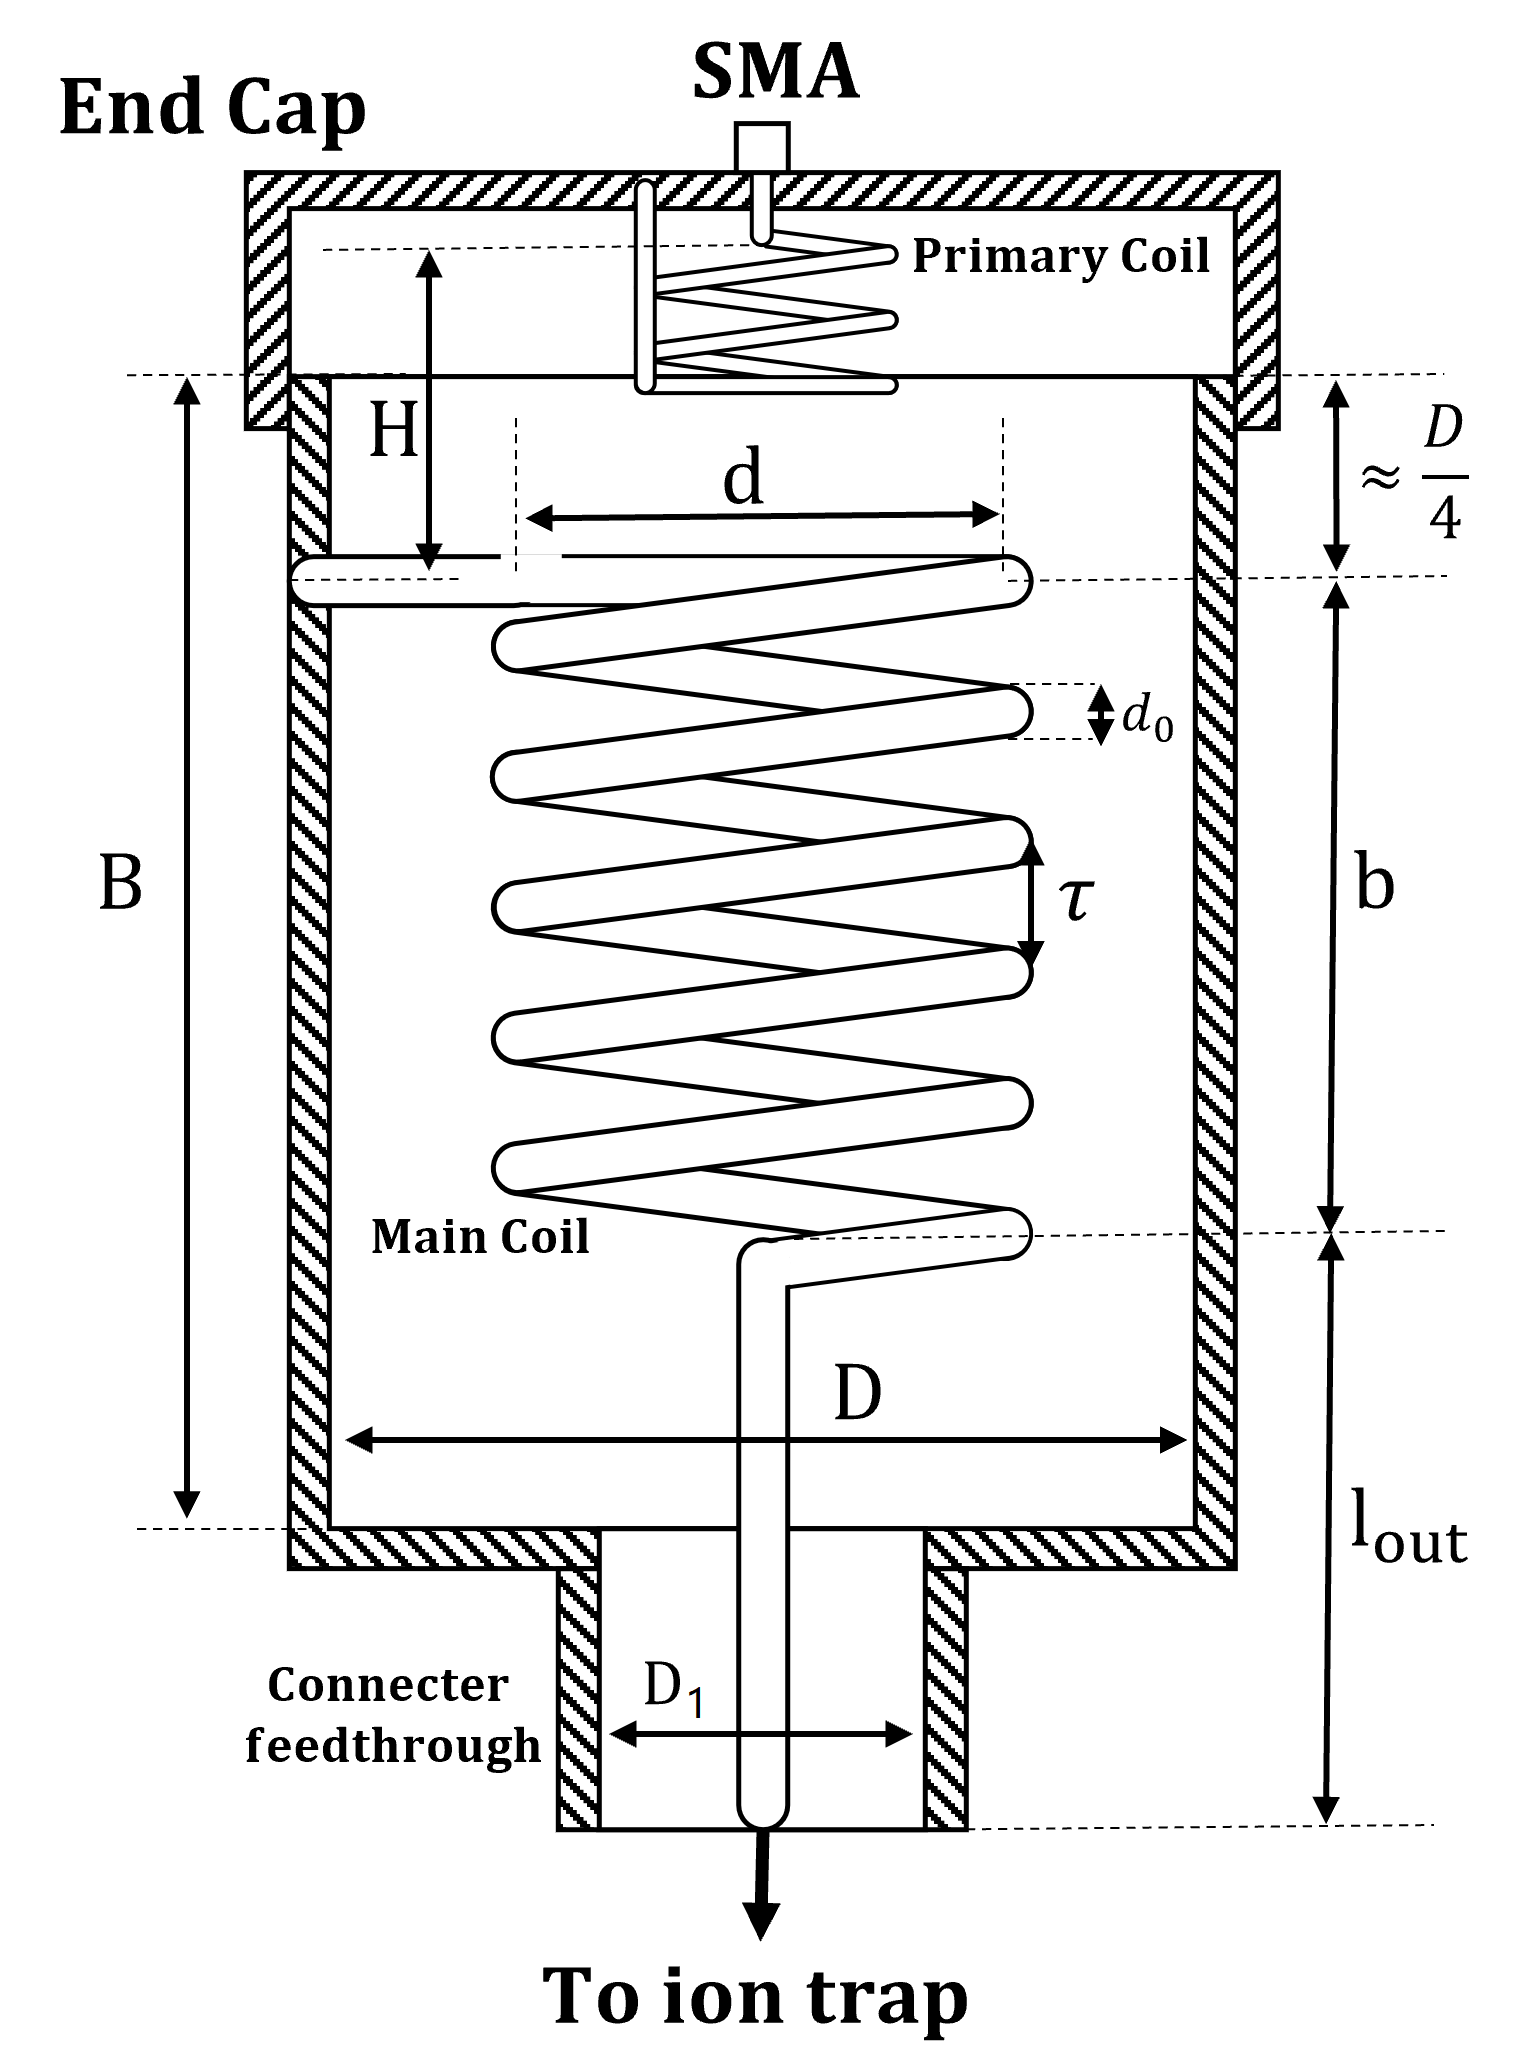
\includegraphics[width=0.5\linewidth]{helical/helical_structure_2d}
    \caption[谐振腔结构平面示意图]{谐振腔结构平面示意图。$H$:耦合线圈底部到主线圈底部的距离;$B$:屏蔽壳侧壁长度;$D$:屏蔽壳内筒直径;$\tau$:主线圈螺距;$d_0$:主线圈线粗;$d$:主线圈直径;$b$:主线圈总长度;$l_{out}$:输出线长度;$D_1$:输出口内直径。\label{fig:helical_structure_2d}}
\end{figure}

\section[螺线管谐振腔的仿真模型]{螺线管谐振腔的仿真模型}

常用的商业化FE仿真工具有ANSYS HFSS、Comsol等,接下来的仿真中我们采用的ANSYS HFSS来研究影响谐振腔$f_0$和$Q$值的各种因素。在HFSS中,有两种方法可以分析3D结构,本征模模式(Eigen-mode)和驱动模式(Driven-mode)。
本征模模式通过分析计算电磁场模式,直接给出谐振频率$f_0$和品质因子$Q$的结果;而驱动模式是通过设置输入和输出射频信号端口,分析和计算\emph{散射参数(Scattering Parameter, SP)},与实验更具可比性。
这两种模式都可以用来模拟螺线管谐振腔,但本征模法更常用于谐振器设计,驱动模式在一般仿真中更为频繁。因为驱动模式得到的结果可以直接与实际实验结果做比对,在接下来的仿真研究中我们默认使用这种方法来进行仿真(特别说明的情况除外)。
请注意,由于阻抗匹配网络损耗\cite[]{Gandolfi_Niedermayr_Kumph_Brownnutt_Blatt_2012},驱动模式中品质因子$Q$的结果大约是本征模结果的一半。

我们在仿真软件中构建了与实际谐振器相同的一个3D模型。模型结构示意图如图\ref{fig:helical_structure_2d}所示,HFSS中建立的3D模型视图如图\ref{fig:helical_HFSS_3d}所示。
% ,其表面电流密度矢量分布如图\ref{fig:helical_HFSS_field}所示。
在这个3D模型中,除了主线圈和铜壳结构外,它还包括耦合线圈、输出导线$l_{out}$和连接器馈通结构,3D模型的所有实体结构均为紫铜材料。
主线圈与铜屏蔽壳侧壁接触(gnd);在耦合线圈和主线圈设置两个集总端口,耦合线圈作为输入端口,主线圈作为输出端口,如图\ref{fig:helical_HFSS_3d}中黄色的圆片所示。通过调整耦合线圈到主线圈的距离可以实现阻抗匹配,阻抗匹配的目标是使得S参数反射最小,仿真中采用的标准是$S_{11}<-40$dB。仿真结果的后处理与实际实验完全相同,中心频率$f_0$和$Q$因子可以从$S$参数导出。图\ref{fig:helical_HFSS_field}所展示了谐振腔仿真模型的表面电流密度矢量分布,从图中可以看出表面电流主要分布在主线圈上,谐振腔的损耗主要发生在主线圈上。追求更大的谐振腔Q值本质上就是为了减小谐振腔器件损耗的发生,因此主线圈的材料和结构将是谐振腔研究一个重点的对象。一般来说,制作谐振腔材料的电阻率越小,损耗越小,Q值越大。出于成本和易用性原因,本研究中谐振腔统一采用紫铜材料制作。除此之外,影响谐振腔的Q值的因素主要是其几何结构设计。

\begin{figure}
    \centering
    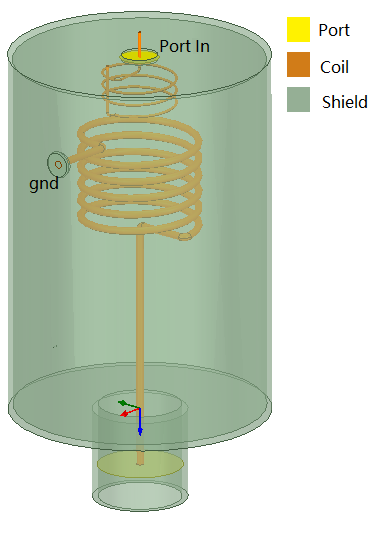
\includegraphics[width=0.4\linewidth]{helical/helical_HFSS_3d}
    \caption[HFSS中建立的3D模型图]{HFSS中建立的3D模型图。黄色圆片表示射频输入和输出端口;橙色部分表示耦合线圈和主线圈,一般采用紫铜材质制作;绿色部分是屏蔽外筒,一般采用紫铜或者黄铜制作。\label{fig:helical_HFSS_3d}}
\end{figure}

\begin{figure}
    \centering
    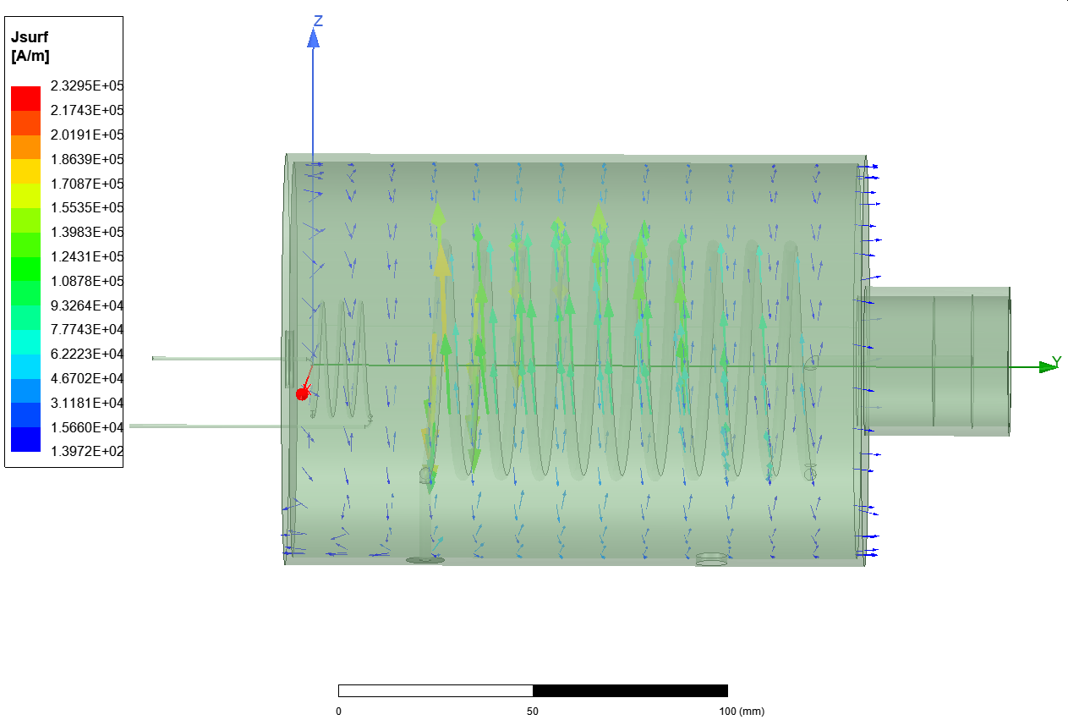
\includegraphics[width=1.0\linewidth]{helical/helical_HFSS_field}
    \caption[HFSS中导出的3D模型表面电流密度矢量图]{HFSS中导出的3D模型表面电流密度矢量图。辅助进行谐振腔的损耗和结构设计分析。从图中可见表面电流主要分布在主线圈上,主线圈的材料和结构是决定谐振腔性能的关键。\label{fig:helical_HFSS_field}}
\end{figure}

离子阱实验中的谐振频率通常在$10-100$ MHz之间,主线圈的典型直径和螺距间距分别为$50-60 $ mm和$5-8$ mm。为了测试HFSS模拟和实验之间的一致性,我们选择了三组几何设置,如表\ref{tb:helical_simulation_parameters}所示。
在每个组中,谐振器具有相似的谐振中心频率,但线圈直径和绕组间距不同,即$30$ MHz、$50$ MHz、$75$ MHz组。
除了正常参数外,我们故意选择一个更大的参数范围,接近线圈直径和绕组间距的极限,比如线圈直径在$30-80$ mm之间(与屏蔽直径$D=103$ mm相比);绕组间距在$4$ mm到$ 18$ mm之间(与导线直径为$d0 = 3$ mm相比)。
关于其它参数,参数$d=48$ mm$/\tau = 7$ mm的初始轮数$N = 5.734$,屏蔽外壳的高度$ B = 136$ mm。螺旋谐振器由网络分析仪Keysight E5063A进行了实验测试。实验测试方案和螺旋谐振器的照片如图\ref{fig:helical_experiment_test}所示。
\begin{table}
    \centering
    \caption[仿真的谐振腔参数设置]{仿真的谐振腔参数设置\label{tb:helical_simulation_parameters}}
    \begin{tabular}{lccccccc}
        %Left\footnote{Note a.}&Centered\footnote{Note b.}&Right\\
        \toprule
        $\#$ & groups & d(mm) & $\tau$(mm) & $f_{HFSS}$(MHz) & $Q_{HFSS}$(1) & f$_{exp}$(MHz) & $Q_{exp}$(1) \\
        \midrule

        1 & \multirow{5}{*}{30 MHz} 	& 40 & 4  & 32.4062 & 565 & 31.7472 & 513   \\
        2 & 						& 80 & 4  & 25.2663 & 346 & 24.8038 & 207   \\
        3 & 						& 60 & 5  & 28.4732 & 639 & 28.3904 & 587   \\
        4 & 						& 50 & 6  & 30.2228 & 650 & 30.6030 & 599   \\
        5 & 						& 80 & 10 & 27.1943 & 354 & 27.6059 & 317   \\
        \midrule
        6 & 50 MHz 					& 48 & 5  & 49.878739 & 708 & 49.2687 & 631   \\
        \midrule
        7 & \multirow{5}{*}{75 MHz} 	& 30 & 4  & 76.4602 & 595 & 76.2748 & 542   \\
        8 & 						& 80 & 4  & 61.2866 & 453 & 60.7942 & 389   \\
        9 & 						& 48 & 7  & 74.9382 & 802 & 75.2466 & 708   \\
        10 & 						& 40 & 14 & 88.4308 & 686 & 88.8163 & 571   \\
        11 & 						& 80 & 18 & 77.9517 & 469 & 78.4634 & 377   \\
        \bottomrule
    \end{tabular}
\end{table}


\begin{figure}
    \centering
    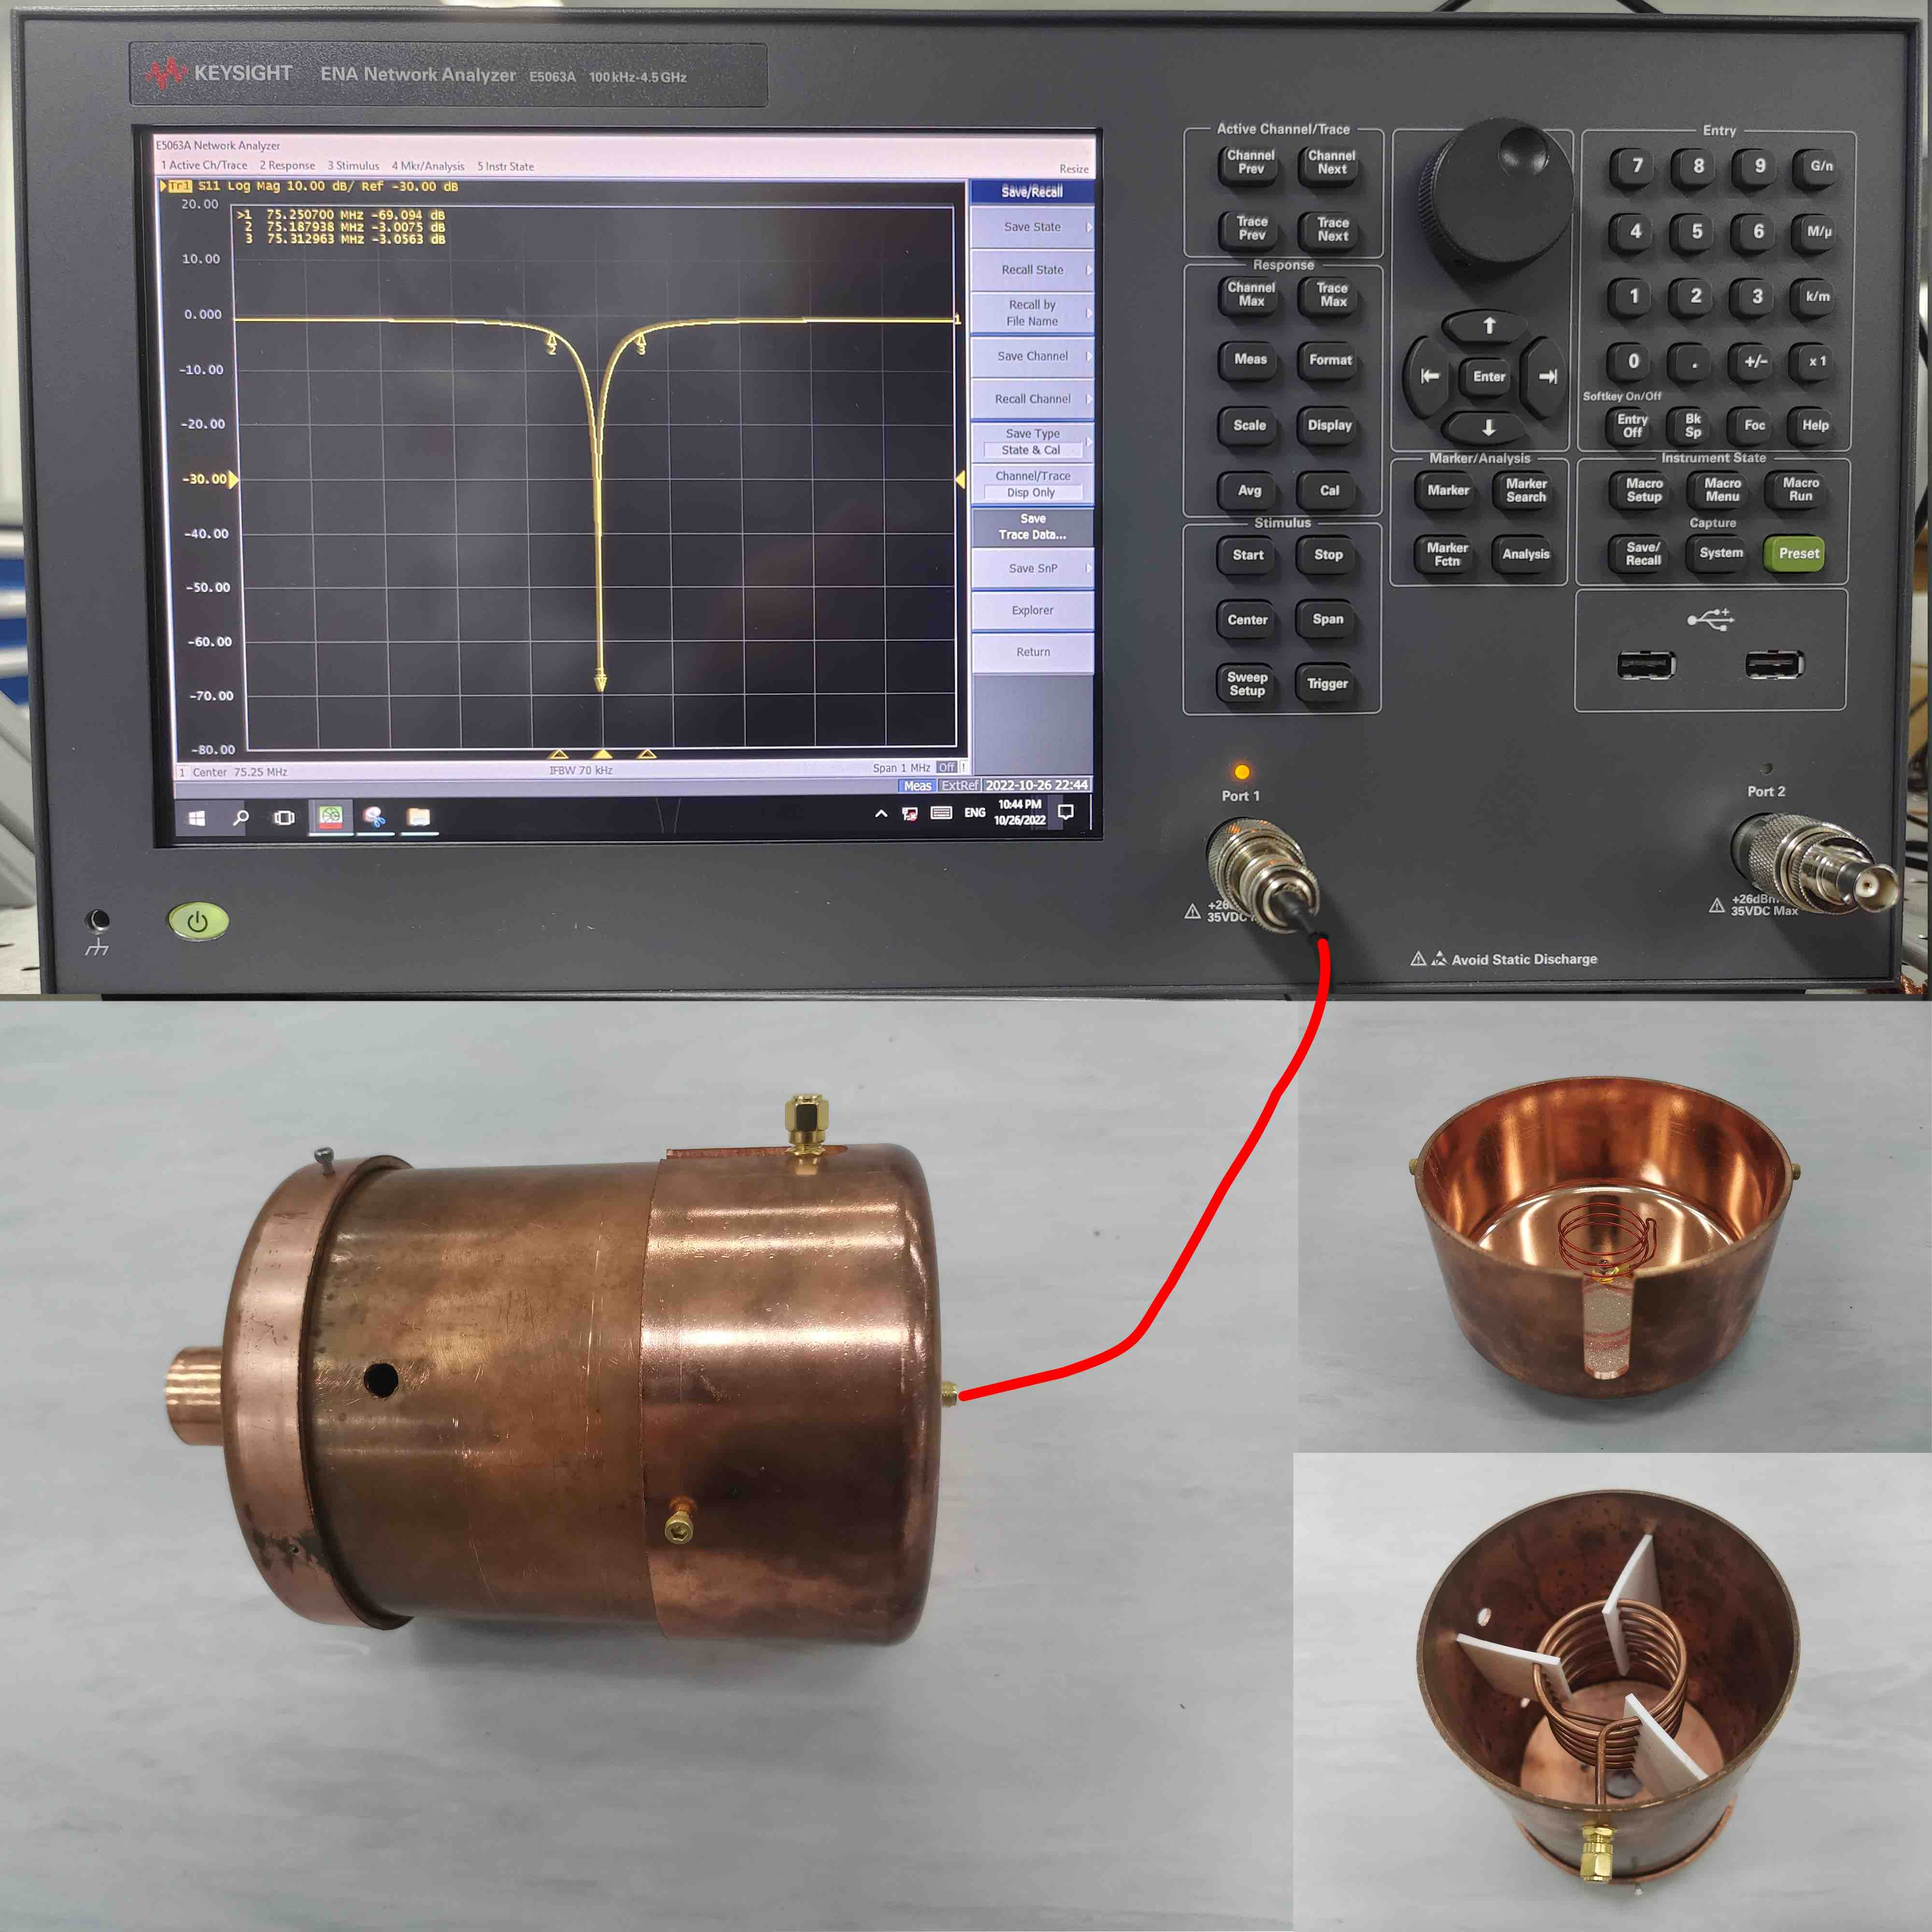
\includegraphics[width=1.0\linewidth]{helical/helical_experiment_test}
    \caption[实际实验的测量方式示意图]{实际实验的测量方式示意图。网络分析仪型号为Keysight E5063A。\label{fig:helical_experiment_test}}
\end{figure}

我们选择在表\ref{tb:helical_simulation_parameters}中的2、6、9三行设置作为示例来比较HFSS模拟和实验的结果,散射参数$S_{11}$的对比结果如图\ref{fig:helical_compares}所示(中心频率平移到相互重合,以便清楚地显示$S_{11}$的差异)。结果中的中心频率差异$\Delta f=f_{exp}-f_{HFSS}$,Q值相对差异$\Delta Q_r=\left(Q_{exp}-Q_{HFSS}\right)/Q_{HFSS}$。实验测试的中心频率差异$\Delta f$和品质因子相对差异$\Delta Q_r$结果和误差棒如图\ref{fig:helical_compares_f_q}所示。误差棒非常小,几乎不可见。频率的最大差异约为$0.7$ MHz。除了一个设置的$\Delta Q_r$外,其它设置的品质因子相对差异$\Delta Q_r$均小于$20\%$,相对较大的$\Delta Q_r$差异的原因可能是由于加工精度、频率和电阻影响。
频率的大小受到电感和电容的影响,电感和电容的具体值由谐振腔的几何结构和材料决定。
电阻受材料和加工过程的影响,例如焊点电阻、金属表面氧化等。此外,我们模拟了我们之前使用的几种主线圈设计,并与实验记录相比,频率差异小于$1$ MHz,$Q$差异小于 $50$。

以上结果表明,仿真方法都能较好地预测实验结果。这验证了HFSS商业软件是帮助设计和预测螺旋谐振器行为的绝佳工具,为谐振腔的研究提供了极大的方便。

\begin{figure}
    \centering
    \subcaptionbox[50 MHz]{50 MHz}{
        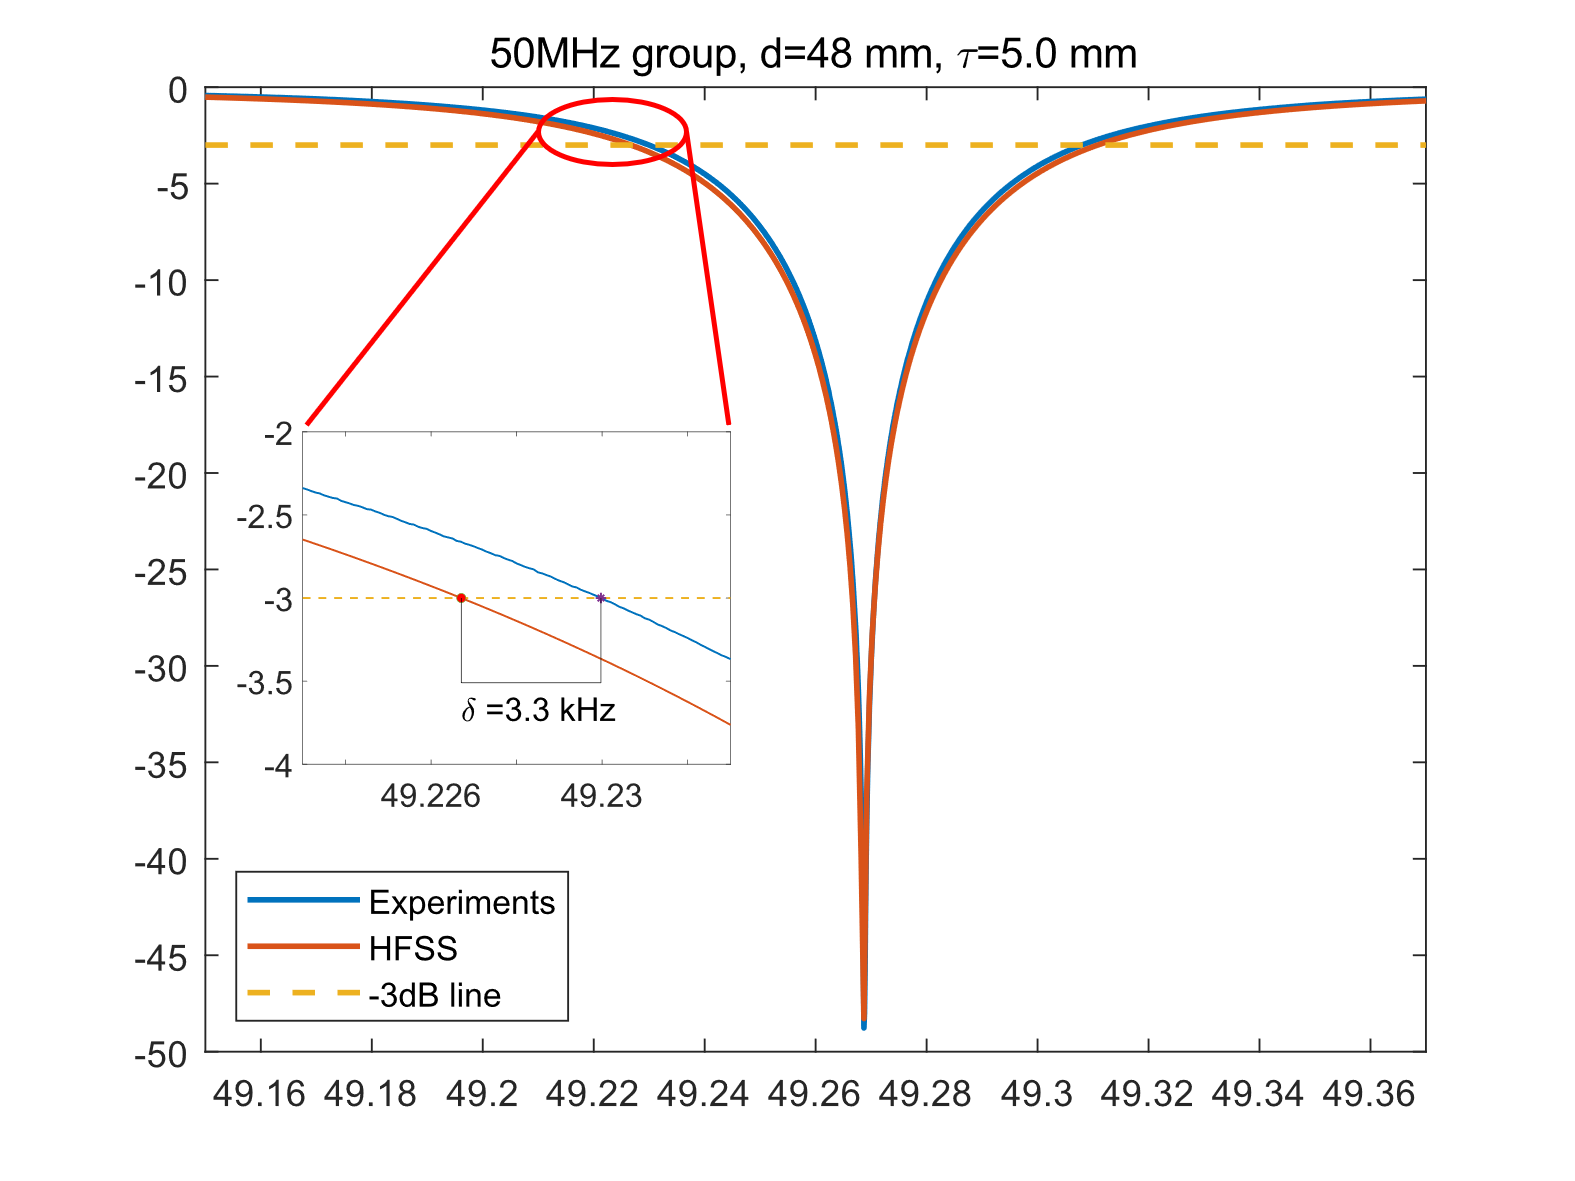
\includegraphics[width=0.8\linewidth]{helical/helical_50MHz_final}
    }
    \subcaptionbox[30 MHz]{30 MHz}{
        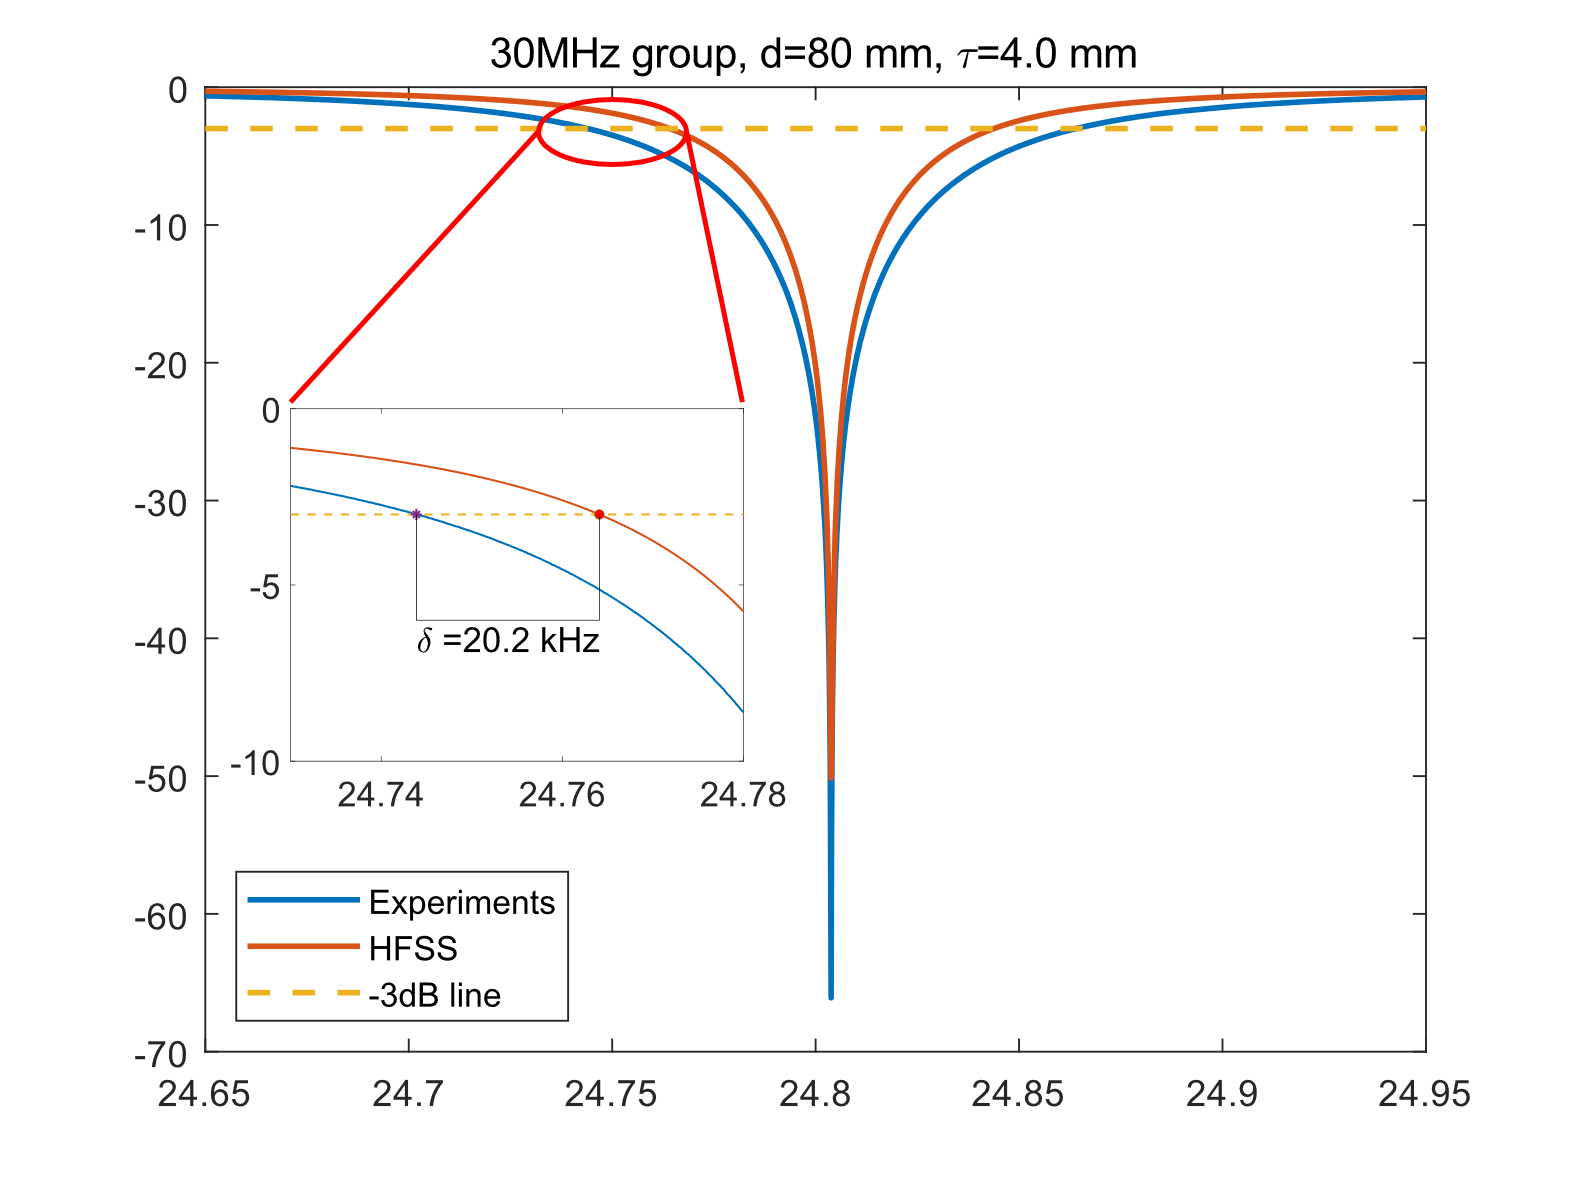
\includegraphics[width=0.46\linewidth]{helical/helical_30MHz_final}
    }
    \subcaptionbox[75 MHz]{75 MHz}{
        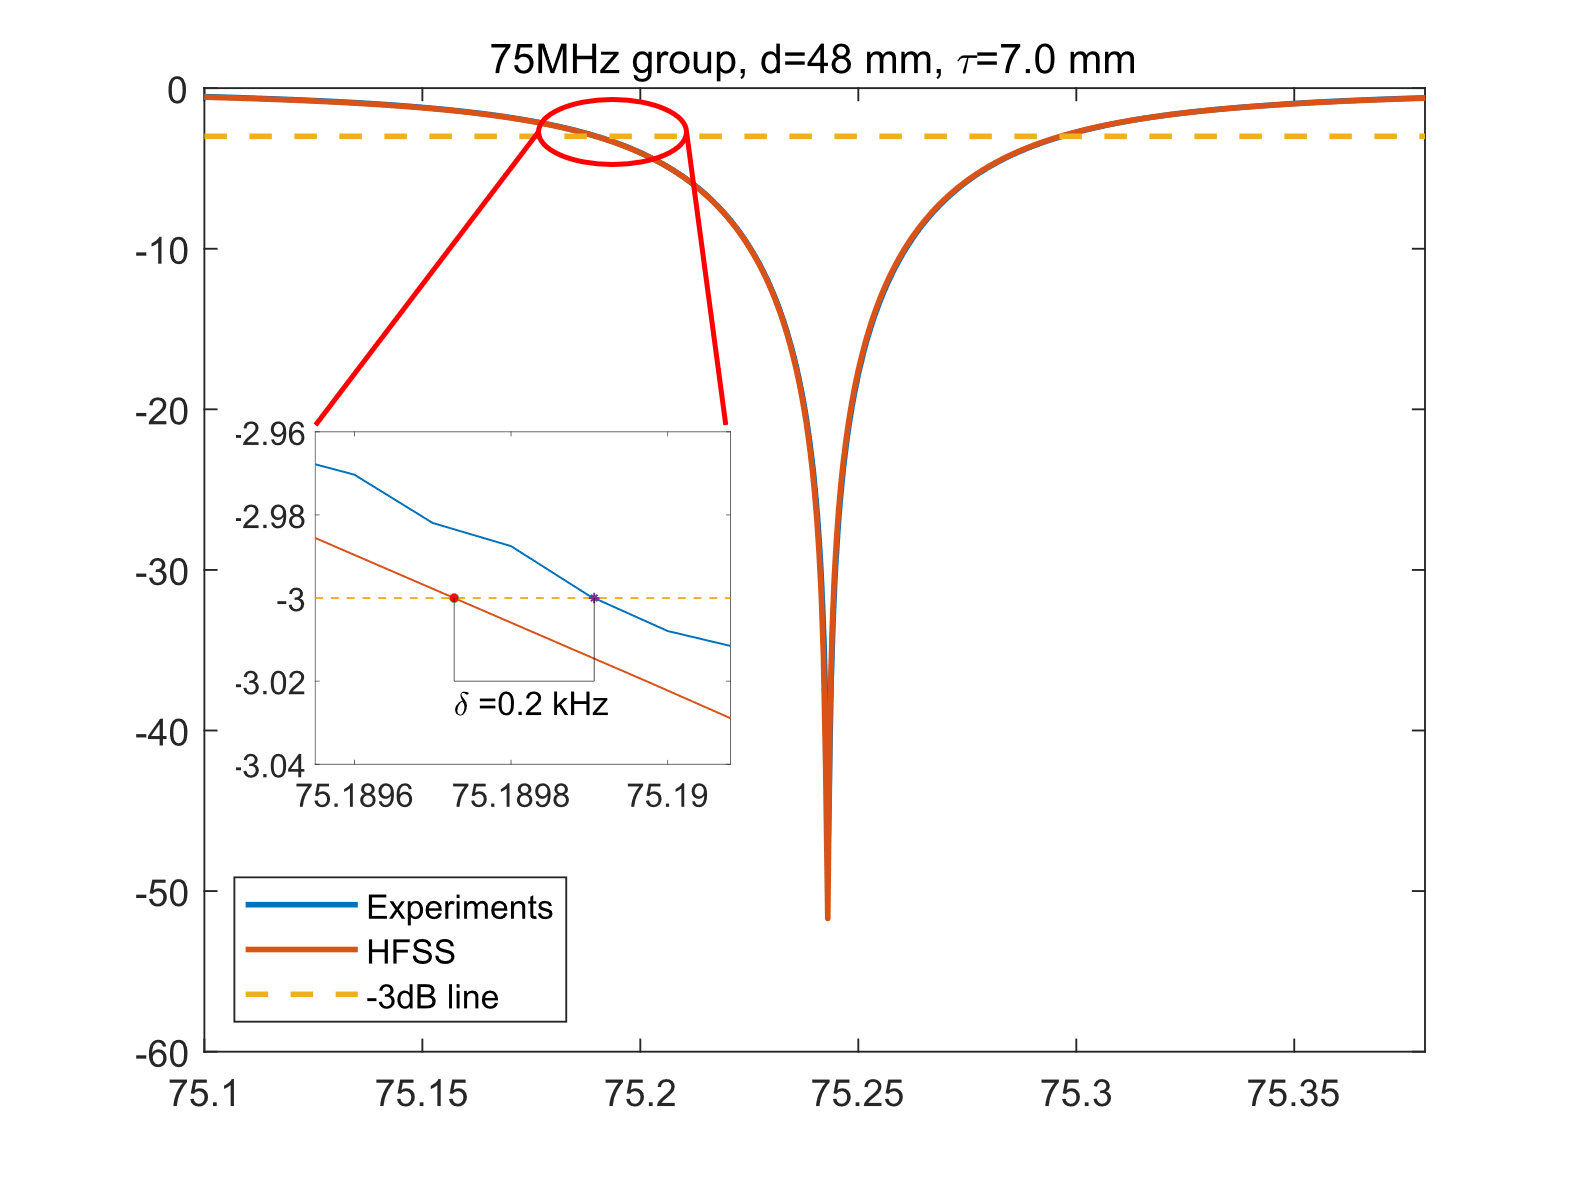
\includegraphics[width=0.46\linewidth]{helical/helical_75MHz_final}
    }
    \caption[谐振腔仿真与实验散射参数结果对比]{谐振腔仿真与实验散射参数$S_{11}$结果对比。其中红色实线为HFSS仿真结果,蓝色实线为实验测得的结果。横坐标为频率(单位MHz),纵坐标为幅度(单位dB)。\label{fig:helical_compares}}
\end{figure}


\begin{figure}
    \centering
    \subcaptionbox[谐振腔仿真与实验频率结果对比]{谐振腔仿真与实验频率结果对比}{
        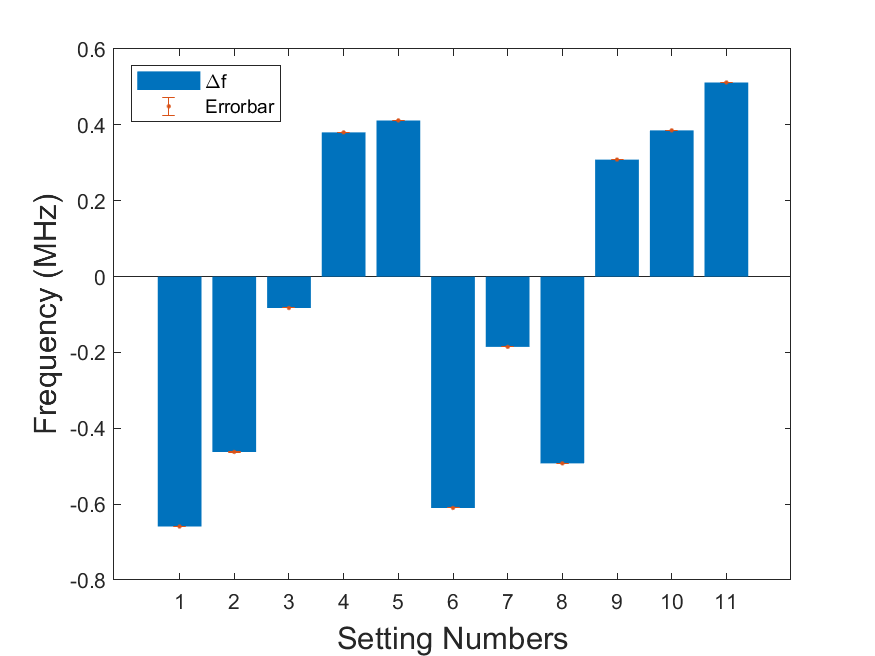
\includegraphics[width=0.48\linewidth]{helical/helical_delta_f}
    }
    \subcaptionbox[谐振腔仿真与实验Q结果对比]{谐振腔仿真与实验Q结果对比}{
        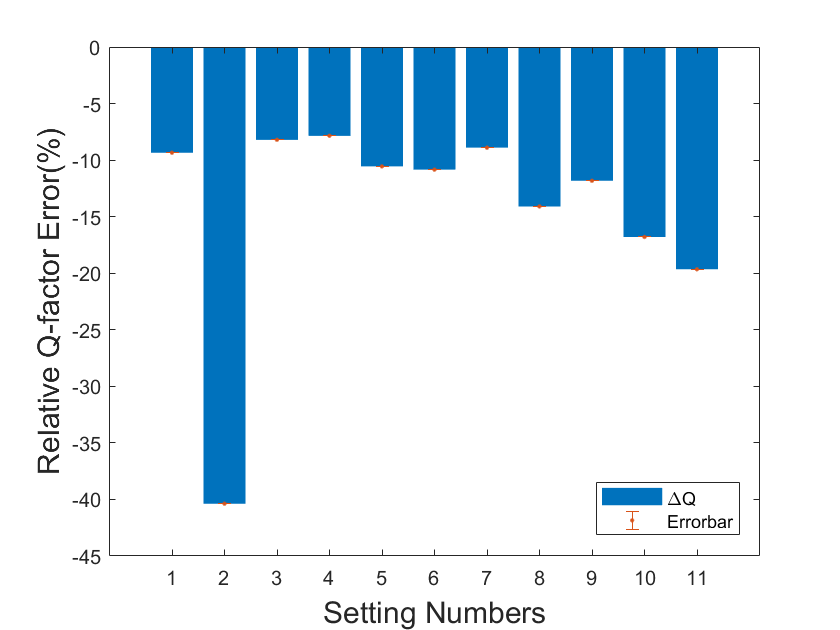
\includegraphics[width=0.48\linewidth]{helical/helical_r_delta_Q}
    }
    \caption[谐振腔仿真与实验频率和Q结果对比]{谐振腔仿真与实验频率和Q结果对比。横坐标为表中对应的序号数,(a)纵坐标为实验与仿真预测的频率结果差异$\Delta f$(单位MHz),(b)纵坐标为实验与仿真预测的品质因子相对差异$\Delta Q_r$(单位\%)。\label{fig:helical_compares_f_q}}
\end{figure}

\section[几何参数对频率和Q的影响]{几何参数对频率和Q的影响}

在离子阱的应用中,螺线管谐振腔最重要的性能是谐振频率和Q因子,具有特定谐振频率和最高$Q$因子的谐振腔是最理想的\cite[]{Siverns_Simkins_Weidt_Hensinger_2012}。
谐振频率和Q可以由以下包含集总参数电感$L$、电容$C$和电阻$R$的公式表达:
\begin{align}
    f&=\frac{1}{2\pi\sqrt{LC}} \label{eq:helical_f_equation}\\
	Q&=\frac{\omega L}{R}=\frac{1}{R}\sqrt{\frac{L}{C}} \label{eq:helical_Q_equation}
\end{align}

对于特定的材料,几何物理参数完全决定了设备的所有特性和等效的集总电路参数。进一步地,频率主要取决于电感和电容两者的比值$L/C$,从几何角度看就是取决于谐振腔主线圈的直径、螺距以及总线长等;在此基础上,$Q$除了跟$L/C$有关外,还与电阻有关。
在之前的研究中,大多数研究人员将线圈直径、绕组间距和主线圈数视为非独立参数\cite[]{Siverns_Simkins_Weidt_Hensinger_2012,Macalpine_Schildknecht_1959}。
然而,在我们的模拟中,我们发现如果主线圈的总长度是固定的,谐振频率将比总导线长度变化小得多,结果如图\ref{fig:helical_fixedwirelength}所示。
这使得谐振频率的控制更容易。一项研究\cite[]{Nandi_Sikdar_Das_Ray_2022}也指出了这种类似的现象,它给出了谐振频率与主线圈长度之间的关系。螺线管谐振腔基本上与四分之一波长谐振器相同。
\begin{figure}
    \centering
    \subcaptionbox[改变主线圈直径参数]{改变主线圈直径参数}{
        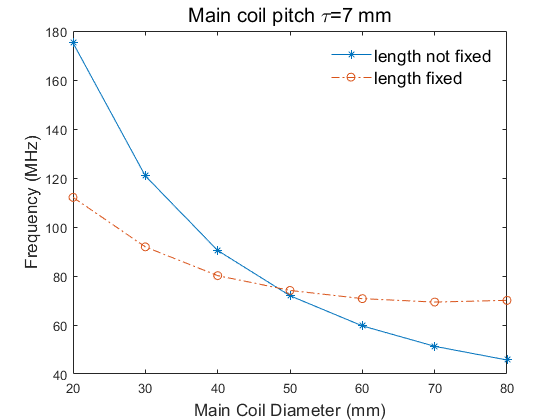
\includegraphics[width=0.48\linewidth]{helical/helical_fixedwirelength_1}
    }
    \subcaptionbox[改变主线圈螺距参数]{改变主线圈螺距参数}{
        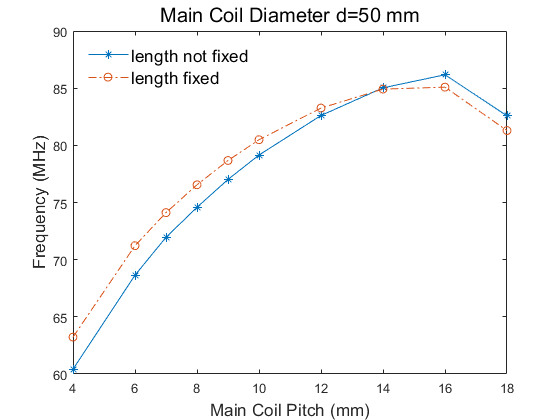
\includegraphics[width=0.48\linewidth]{helical/helical_fixedwirelength_2}
    }
    \caption[固定线长下改变主线圈参数的频率$f_0$变化]{固定线长下改变主线圈参数的频率$f_0$变化。(a)横坐标为主线圈直径$d$(单位mm),(b)主线圈螺距$\tau$(单位mm);纵坐标为频率$F$(单位MHz)。\label{fig:helical_fixedwirelength}}
\end{figure}

在我们的模拟中,主要线圈几何形状设置了两个限制,即固定的总导线长度$l_{total}$和固定的输出线高度$h$:
\begin{align}
    l_{total}&=N\sqrt{(\pi d)^2+\tau^2}+l_{out} \label{eq:helical_fixed_constraints_1}\\
	h&=N\tau+l_{out} \label{eq:helical_fixed_constraints_2}
\end{align}

因此,频率在$d=20$ mm到$d=80$ mm时平均变化约为$0.701$ MHz/mm;虽然绕组间距效应不那么明显,但频率在$\tau=4$ mm到$\tau=118$ mm时平均变化约为$1.29$ MHz/mm。这种现象有助于分离几何效应和频率变化之间$ Q $因子改进的原因。接下来的几节将在这些预设下,研究几个几何参数的效应来设计所需的频率$f_0$和$Q$因子。
\subsection[主线圈几何参数的影响]{主线圈几何参数的影响}

为了研究对谐振频率$f_0$和$Q$因子的几何效应,基于表\ref{tb:helical_simulation_parameters}中第9行的参数,对几组主线圈参数进行设置和模拟。
主线圈的直径和间距设置为双参数扫描;直径从$30-80$ mm,步长为$10$ mm;螺距设置为$4-18$ mm,步长为$2$ mm。
这些模拟的结果给出了一个谐振频率$f_0$和$Q$因子的几何效应图,将其绘制为等高线图,如图\ref{fig:helical_contour}所示。左上角的白色三角形是参数禁止区,因为主线圈参数不满足约束公式\eqref{eq:helical_fixed_constraints_1}和\eqref{eq:helical_fixed_constraints_2}。
使用一组确定的参数($d$和$\tau$),可以近似在这个等高线图上立即读出谐振频率$f_0$和$Q$因子,如图中红点代表表\ref{tb:helical_simulation_parameters}中第9行的参数设置。

\begin{figure}
    \centering
    \subcaptionbox[螺线管谐振腔$f_0$值等高图]{螺线管谐振腔$f_0$值等高图\label{fig:helical_contour_f}}{
        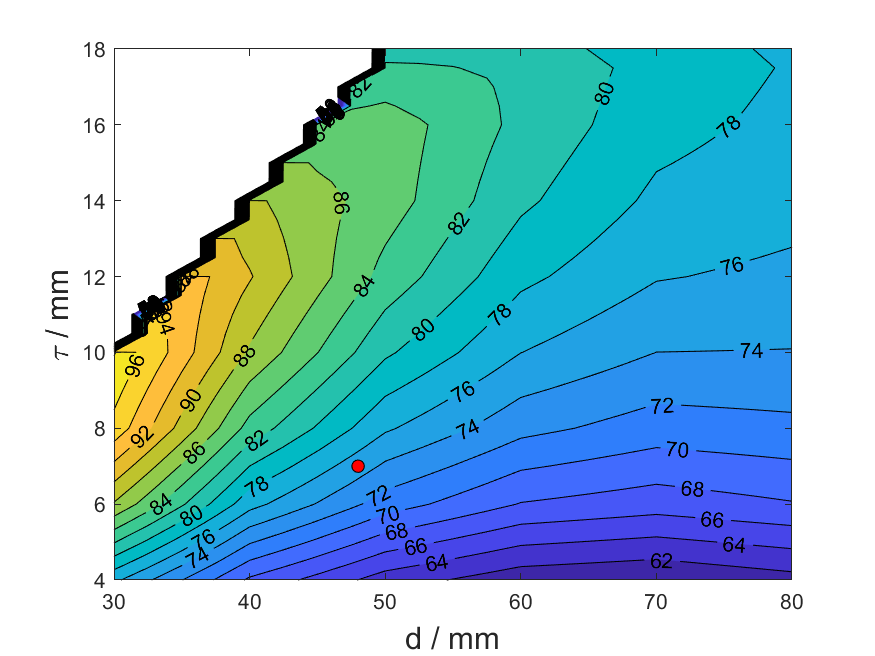
\includegraphics[width=0.48\linewidth]{helical/helical_contour_f}
    }
    \subcaptionbox[螺线管谐振腔$Q$值等高图]{螺线管谐振腔$Q$值等高图\label{fig:helical_contour_Q}}{
        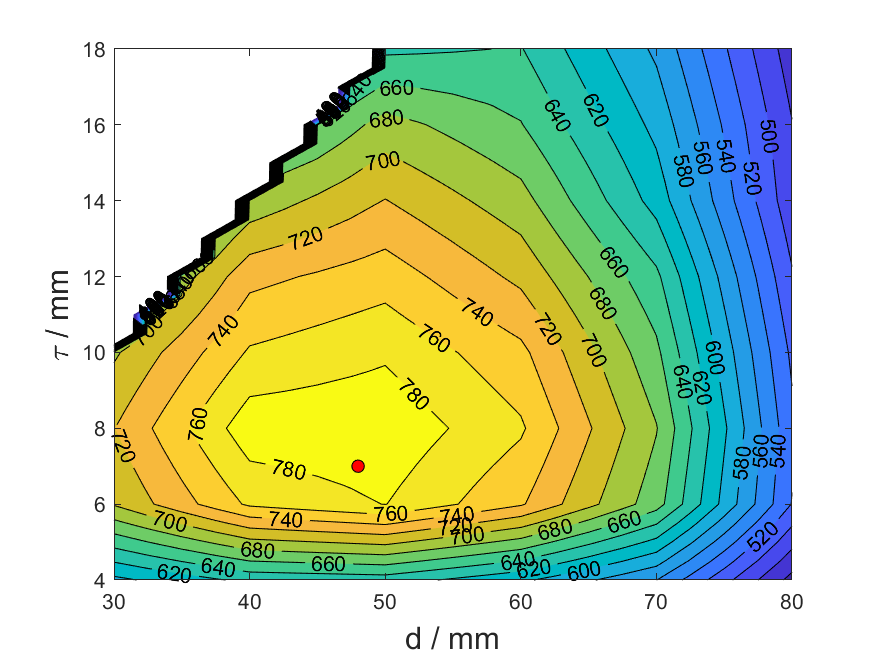
\includegraphics[width=0.48\linewidth]{helical/helical_contour_Q}
    }
    \caption[螺线管谐振腔$f_0$、$Q$值等高图]{螺线管谐振腔$f_0$、$Q$值等高图。横坐标为主线圈直径$d$(单位mm),纵坐标为主线圈螺距$\tau$(单位mm)\label{fig:helical_contour}}
\end{figure}

在图\ref{fig:helical_contour_f}中,频率$f_0$在绝大部分地方随着$\tau$的减小而减小。随着主线圈直径$d$的增加,电感$L$会先慢慢增加(当$d$较小时)然后减小(当$d$较大时)。同时,$C_c$和$C_s$单调地增加。因此在这个过程中频率会先急剧下降然后慢慢下降。参考频率计算公式\eqref{eq:helical_f_equation}和文献\cite[]{Siverns_Simkins_Weidt_Hensinger_2012,Macalpine_Schildknecht_1959}中的电感$L$和电容$C = C_c +C_s$计算公式:
\begin{align}
    L&=39.37b\frac{0.025d^2(1-(\frac{d}{D})^2)}{\tau^2} &\mu \textnormal{H/m} \label{eq:helical_L} \\
	C_c&=d(11.26\frac{b}{d}+8+\frac{27}{\sqrt{b/d}})  &\textnormal{pF/m} \label{eq:helical_C_c}\\
	C_s&=39.37b\frac{0.75}{lg(D/d)} &\textnormal{pF/m} \label{eq:helical_C_s}
\end{align}

然而,在左上和右下角,有两个非单调异常区域。一种是在大$d$和小$\tau$参数区(右下区域)。
频率等高线不是单调的,随着$d$的增大等高线向下弯曲。
这是因为当单独改变$d$时$L$有一个最大值,并且由$\tau$导致的$L$变化不足以逆转这个最大值附近的影响。另一处是在小$d$和大$\tau$参数区(左上区域)。在这里频率等高线也不是单调的,随着$\tau$的增大等高线向左弯曲(如果是将$\tau$作为横轴则是向下弯曲)。这是因为当$\tau$过大时会螺线圈会更加接近输出端会更加接近屏蔽壳引入较大的侧壁电容$C_s$而增大$\tau$带来的电感减少效应不足以抵消,从而导致频率未能随$\tau$单调增加。

对于$Q$的变化,如图\ref{fig:helical_contour_Q}所示,它具有一个明显的最大值。可见选择合适的$d$和$\tau$是十分重要的。图中$Q$的最大值位置约在$d=48$ mm,$\tau=7.3$ mm处,最大值$Q$约为$810$。图中红点表示了表\ref{tb:helical_simulation_parameters}中第9行的参数的$Q$值结果。

在图\ref{fig:helical_contour}的$ f_0,\ Q $结果图的帮助下,可以直接读出具有特定几何参数设置的任何$f_0$和$Q$结果。该图还可以帮助谐振腔设计和确定的$f_0$和$Q$。
此外,沿$d$或$\tau$方向任意点的偏导数将给出线圈参数对频率和$Q$的敏感性。几何参数对$f,\ Q$的敏感性决定了线圈的加工精度,以及实验误差范围。
以图\ref{fig:helical_contour}中的红点参数为例,计算线圈$d$和$\tau$灵敏度,结果如表\ref{tb:helical_d_tau_sensitivity}所示。
从结果中可以看出,灵敏度$d$的结果值小于$\tau$的结果值。因此,在加工过程中,$\tau$大小的偏差更有可能对 $f,\ Q$产生影响,值得更多地关注。

\begin{table}
    \centering
    \caption[谐振腔对主线圈直径和螺距参数的敏感性]{谐振腔对主线圈直径和螺距参数的敏感性\label{tb:helical_d_tau_sensitivity}}
    \begin{tabular}{ccccc}
        \toprule
        改变对象 & 变化范围 (mm) & 频率敏感度(MHz/mm) & Q敏感度(/mm) \\
        \midrule
        直径$d$  & [-1,1] & $\approx$-0.606 & $\approx$ 0.4\\
        螺距$\tau$  & [0, 0.5] & $\approx$ 2.988 & $\approx$ 23.491 \\
        线圈轴向偏移 & [-2, 2] & $\approx$ -0.049 & $\approx$ 0.185\\
        线圈径向偏移 & [-2, 2] & $\approx$ 0.034 & $\approx$ -0.4904\\
        \bottomrule
    \end{tabular}
\end{table}

除了研究$f,\ Q$的独立参数变化效应外,我们还研究了主线圈平移对$f,\ Q$的影响,即沿径向或轴向。结果如图\ref{fig:helical_bias_axial}、图\ref{fig:helical_bias_radial_gndalong}、图\ref{fig:helical_bias_radial_gndperpendicular}和表\ref{tb:helical_d_tau_sensitivity}所示。
从结果可以看出,主线圈的轴向平移和径向平移对$f,\ Q$影响不大。平移对$f,\ Q$的影响远小于几何参数 ($d,\ \tau$) 变化效应。因此,我们需要更多地关注加工过程中主线圈的俯仰精度,以获得更一致的实验结果。

\begin{figure}
    \centering
    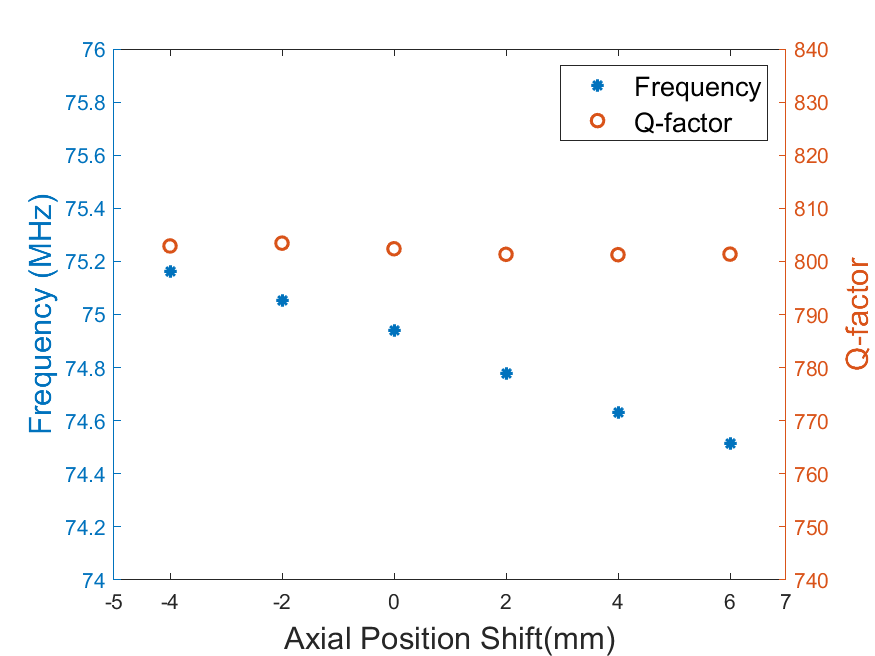
\includegraphics[width=0.8\linewidth]{helical/helical_bias_axial}
    \caption[谐振腔仿真与实验结果对比——主线圈轴向偏移]{谐振腔仿真与实验结果对比——主线圈轴向偏移。\label{fig:helical_bias_axial}}
\end{figure}

\begin{figure}
    \centering
    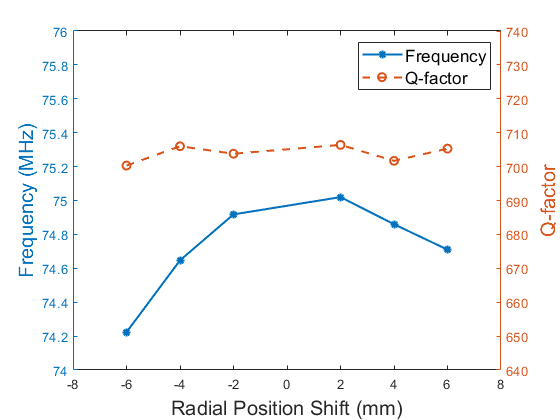
\includegraphics[width=0.8\linewidth]{helical/helical_bias_radial_gndalong}
    \caption[谐振腔仿真与实验结果对比——主线圈径向偏移(垂直于接地端)]{谐振腔仿真与实验结果对比——主线圈径向偏移(垂直于接地端)。\label{fig:helical_bias_radial_gndalong}}
\end{figure}

\begin{figure}
    \centering
    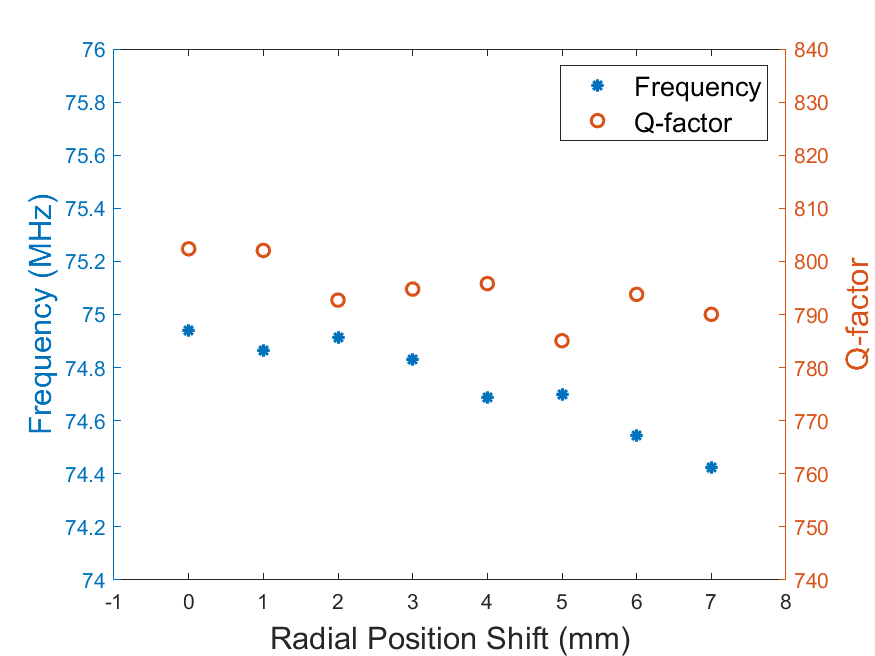
\includegraphics[width=0.8\linewidth]{helical/helical_bias_radial_gndperpendicular}
    \caption[谐振腔仿真与实验结果对比——主线圈径向偏移(垂直于接地端)]{谐振腔仿真与实验结果对比——主线圈径向偏移(垂直于接地端)。\label{fig:helical_bias_radial_gndperpendicular}}
\end{figure}


% \begin{figure}
%     \centering
%     \caption[谐振腔仿真与实验散射参数结果对比]{谐振腔仿真与实验结果对比。(a)横坐标为主线圈轴向偏移距离(单位mm),(b)主线圈平行于接地端径向偏移(单位mm),(c)主线圈垂直于接地端径向偏移(单位mm)。\label{fig:helical_main_coil_compares}}
%     \subcaptionbox[主线圈轴向偏移]{主线圈轴向偏移\label{fig:helical_bias_axial}}{
%         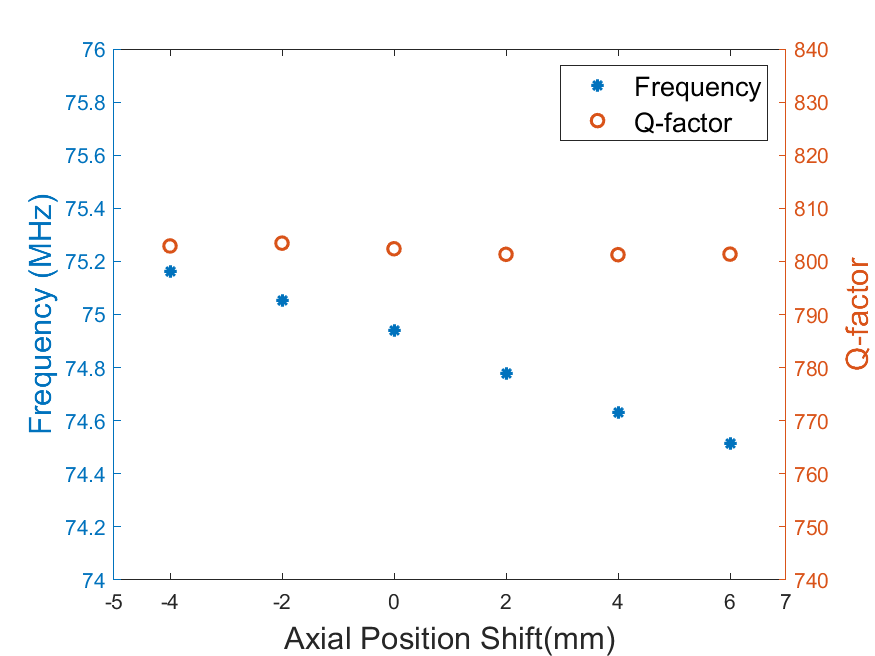
\includegraphics[width=0.8\linewidth]{helical/helical_bias_axial}
%     }
%     \subcaptionbox[主线圈径向偏移(平行于接地端)]{主线圈径向偏移(平行于接地端)}{
%         %0.46 for two
%         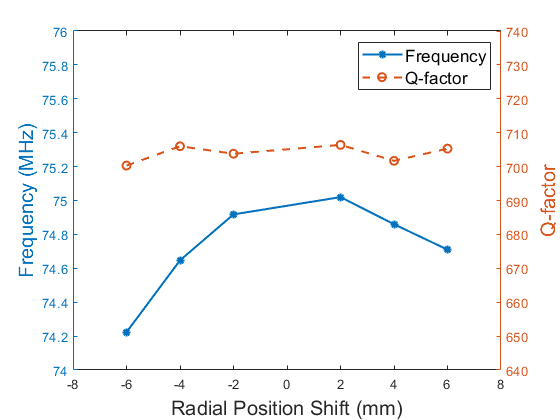
\includegraphics[width=0.8\linewidth]{helical/helical_bias_radial_gndalong}
%     }
%     \subcaptionbox[主线圈径向偏移(垂直于接地端)]{主线圈径向偏移(垂直于接地端)}{
%         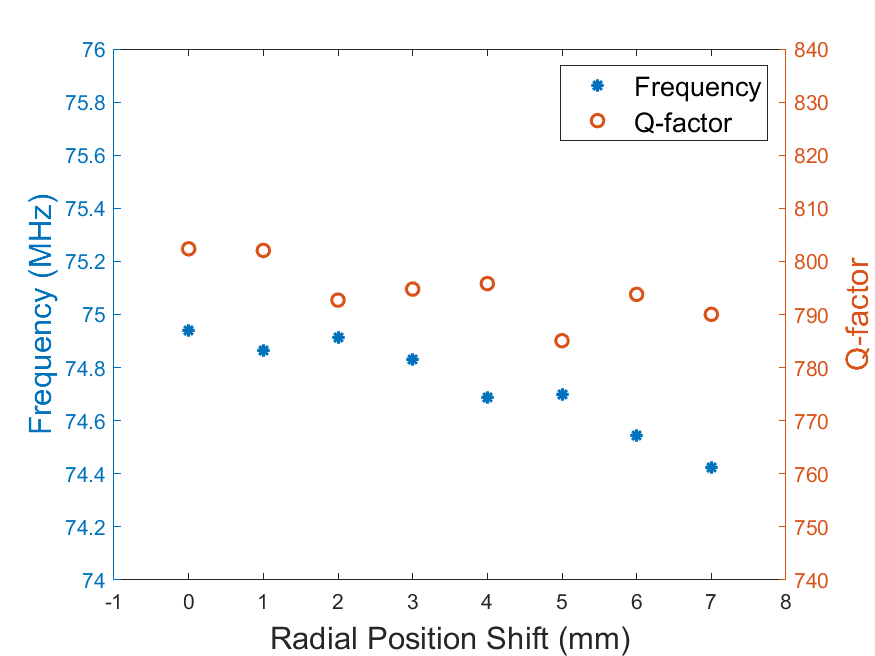
\includegraphics[width=0.8\linewidth]{helical/helical_bias_radial_gndperpendicular}
%     }
% \end{figure}


\subsection[输出线参数的影响]{输出线参数的影响\label{section:helical_output_wire}}
在我们的模拟中,我们发现输出导线长度对谐振$f,\ Q$有很大的影响。与之前的固定线长情况不同,这里我们不再做式\eqref{eq:helical_fixed_constraints_1}和式\eqref{eq:helical_fixed_constraints_2}的约束。
主线圈直径及其螺距保持在相同的长度,独立改变输出导线$l_{out}$的总长度,其中$l_{out} = l_{lout1} + l_{lout2}$。
$l_{out1}$和$l_{out2}$分别是屏蔽外壳中的输出线和连接器馈通部分的输出线,如图\ref{fig:helical_lout_2}所示。


\begin{figure}
    \centering
    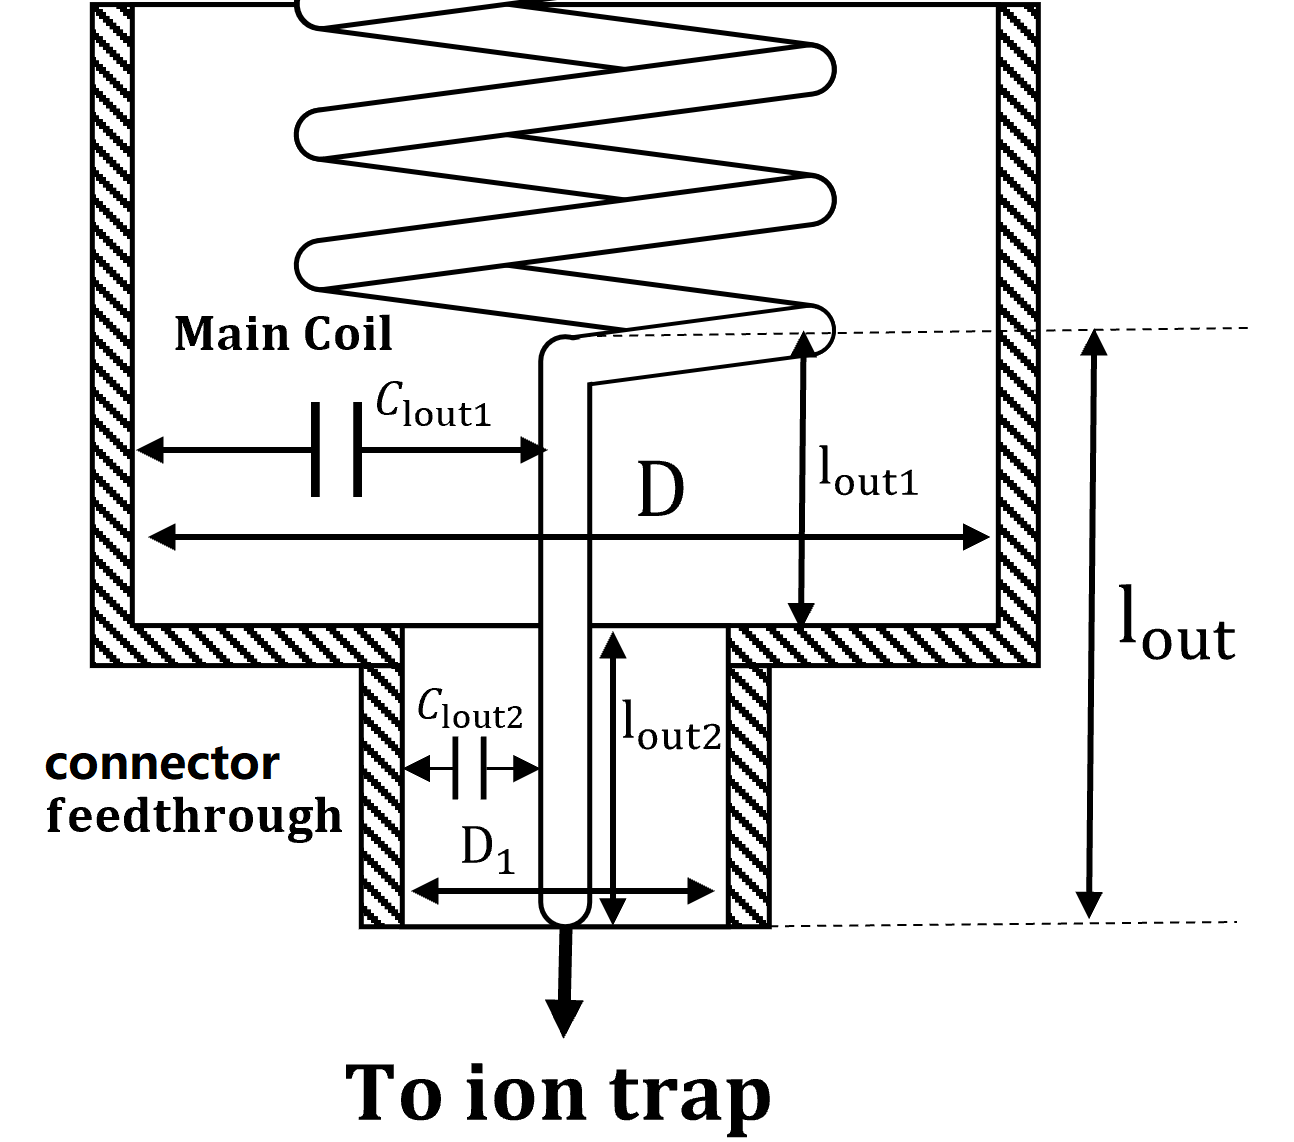
\includegraphics[width=0.5\linewidth]{helical/helical_lout_2}
    \caption[输出线部分示意图]{输出线部分示意图。$l_{out1}$:输出线在屏蔽壳内部分的长度;$C_{lout1}$:输出线在屏蔽壳内部分的电容;$l_{out2}$:输出线在输出端口内部分的长度;$C_{lout2}$:输出线在输出端口内部分的电容;$D$:屏蔽壳内直径;$D_1$:输出端内直径。\label{fig:helical_lout_2}}
\end{figure}

仿真结果如图\ref{fig:helical_lout_1}所示。随着输出导线长度的增加,谐振频率下降。$Q$随着谐振频率的减小而减小,两者成正比,与式\eqref{eq:helical_Q_equation}具有相同的关系。这主要是输出线引入额外电容而对电阻和电感影响较小导致的。

\begin{figure}
    \centering
    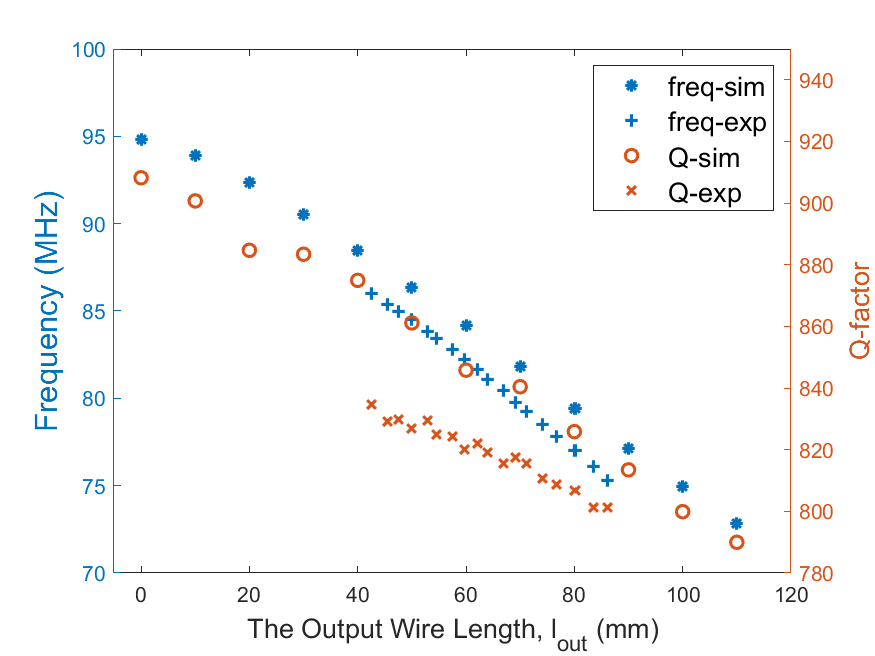
\includegraphics[width=0.8\linewidth]{helical/helical_lout_1}
    \caption[输出线部分影响]{输出线部分影响。横坐标为输出线长$l_{out}$(单位mm),蓝色‘*’标和‘+’标分别为仿真和实验的频率$F$(单位MHz,对应左侧纵坐标),橙色‘o’标和‘x’标分别为仿真和实验的品质因子$Q$(单位1,对应右侧纵坐标)。\label{fig:helical_lout_1}}
\end{figure}

为了验证仿真结果,我们进行了输出导线长度切割实验,测量了输出导线长度和器件谐振频率$f_0$和$Q$。结果如图\ref{fig:helical_lout_1}所示。实验与模拟的频率差约为$2$ MHz,实验测量的$Q$数据比模拟低约$150$。为了在同一图中绘制$ Q $数据,实验$ Q $数据偏移了$ 100$。除了偏移之外,频率$f_0$和$ Q $都与其对应的数据一致。该结果再次表明了仿真结果的可信度。

文献\cite[]{Gandolfi_Niedermayr_Kumph_Brownnutt_Blatt_2012,Macalpine_Schildknecht_1959, Deng_Sun_Yuan_Xu_Zhang_Lu_Luo_2014}之前研究中的理论预测和实验之间的大频率误差可能来自于忽略输出线电容\cite[]{Nandi_Sikdar_Das_Ray_2022, Batra_Panja_De_Roy_Majhi_Yadav_Sen_Gupta_2017}。我们给出了改进的LCR电路模型和一种新的电容评估公式来估计频率。与 HFSS 仿真结果相比,我们的新模型的频率预测有了很大的提高,更多细节见第\ref{section:helical_theory_model}节。

\subsection[屏蔽外壳参数的影响]{屏蔽外壳参数的影响}
\begin{figure}
    \centering
    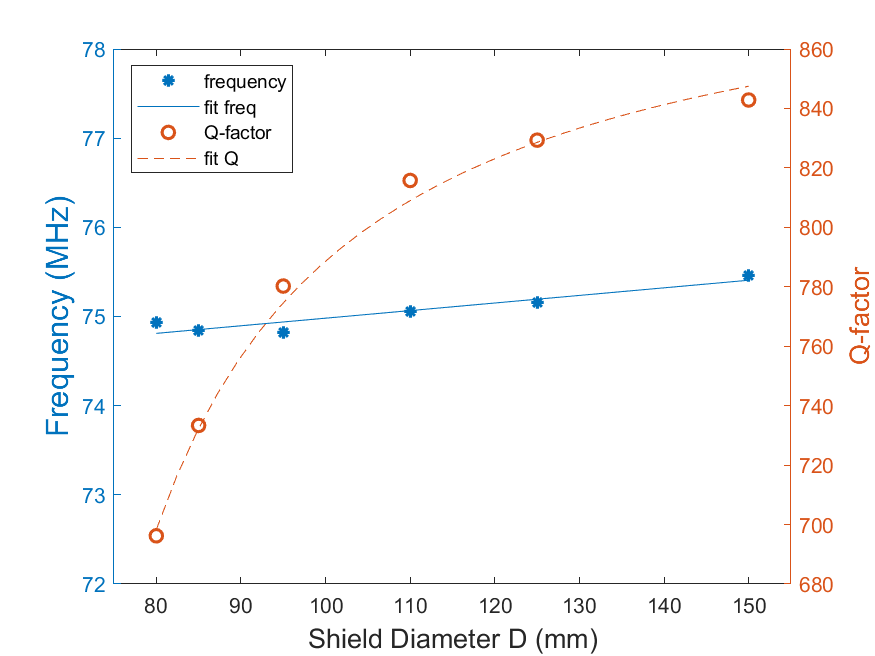
\includegraphics[width=0.8\linewidth]{helical/helical_shield_diameter}
    \caption[屏蔽外壳的影响]{屏蔽外壳的影响,横坐标为屏蔽壳内直径$D$(单位mm),纵坐标为频率$F$(单位MHz)。蓝色实线和‘*’标点为频率(单位MHz,对应左侧纵坐标),橙色虚线和‘o’标点为品质因子Q(单位1,对应右侧纵坐标)。\label{fig:helical_shield_diameter}}
\end{figure}

铜屏蔽外壳完成了电流回路,定义了螺旋谐振腔中的电磁场边界条件。屏蔽外壳和主线圈形成电容$C_s$,因此屏蔽的直径对谐振频率有影响。屏蔽外壳可以屏蔽和减少电磁场辐射耗散,因此谐振器将具有高$Q$因子。在这里,通过数值模拟研究了屏蔽外壳直径$ D $对频率$f_0$和$ Q $因子的影响。结果如图\ref{fig:helical_shield_diameter}所示,当屏蔽直径$ D $增加时,频率$f_0$和$ Q $因子都会增加。频率变化很小,而$ Q $因子首先快速增长,然后逐渐减慢。频率的微弱增加是由于侧壁电容随着屏蔽外壳$D$的增大而减小。$Q$因子的增加是因为屏蔽直径越大,电场强度越小,屏蔽电流越小,电阻相等,耗散越小。因此为了获得更大的$Q$,在合理的设备尺寸下将首选较大的屏蔽直径。

屏蔽外壳高度的影响与相对于外壳沿轴向移动主线圈位置并相应地调整端帽位置相同。结果如图\ref{fig:helical_bias_axial}所示。屏蔽高度对频率$f_0$和$Q$因子的影响很小。

\subsection[耦合线圈参数的影响]{耦合线圈参数的影响}

耦合线圈是螺线管谐振腔的一个有趣部分。通过调节耦合线圈的形状和位置可以满足阻抗匹配条件,实现最佳耦合以最小化散射参数$S_{11}$。然而,据我们所知,以前还没有耦合线圈几何形状影响的具体相关研究。在这里,数值模拟方法提供了研究这些问题的机会。

\begin{figure}
    \centering
    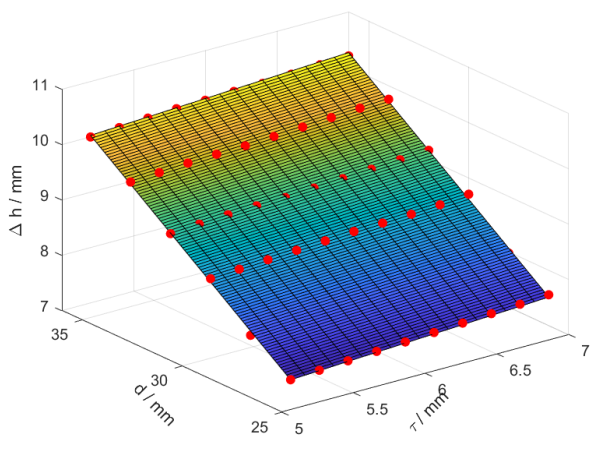
\includegraphics[width=0.8\linewidth]{helical/helical_primary_coil}
    \caption[耦合线圈的影响]{耦合线圈的影响。$\Delta h$:耦合线圈和主线圈之间的距离(单位mm);$d$:耦合线圈的直径(单位mm);$\tau$:耦合线圈的螺距(单位mm)。\label{fig:helical_primary_coil}}
\end{figure}

为了研究主线圈形状效应,我们在其他参数满足表\ref{tb:helical_simulation_parameters}中第9行的情况下,模拟了各种耦合线圈尺寸(耦合线圈直径$d_1$和螺距$\tau_1$)及其轴向位置,并试图满足阻抗匹配。
对于每个耦合线圈(直径$d_1$和螺距$\tau_1$),扫描和优化耦合线圈在轴向的位置,以实现最小耦合反射$S_{11}$。
如果$S_{11}$系数可以达到$-45$dB或更低,认为阻抗匹配过程完成,同时记录耦合线圈轴向位置。仿真结果如图\ref{fig:helical_primary_coil}所示。
$x$轴和$y$轴分别为直径$d_1$和俯仰$\tau_1$,$z$轴为耦合线圈达到最佳耦合条件时的轴向位置。
结果表明,所有$ d_1,\ \tau_1 $参数设置都具有最佳的耦合位置$ \delta_1$,几乎所有数据点($d_1,\tau_1\delta_1$)都位于同一平面表面上。
这意味着耦合线圈的绝对形状对于实现阻抗匹配过程并不重要。在合理范围内,总可以通过调整耦合线圈轴向位置来补偿耦合线圈的所有变形。

\section{谐振腔耦合过程特性}
谐振腔的实际使用离不开一个十分重要的过程,即阻抗匹配,我们一般称为耦合。经验上来看,我们知道可以通过移动耦合线圈和主线圈之间的距离或者改变耦合线圈的形状来实现耦合。一般来说实践上我们更倾向于改变耦合线圈和主线圈之间的距离的方式来实现耦合,存在一个最优距离使得匹配最佳,两者的距离太近或者太远都无法实现最佳匹配。只有在最佳匹配的时候射频功率透过谐振腔的传输率才能达到最大。在耦合的过程中谐振腔的最佳耦合频率会发生微小的偏移,而Q值则会发生较大的变化。值得注意的是,我们发现耦合过程中最佳耦合频率点和Q值的变化并不像最佳耦合点一样有最有值,如图\ref{fig:helical_coupling_delta}所示,它们是随着耦合距离单调变化的。也就是说,在最佳耦合点左右两侧,虽然透过率都会下降,但是两侧的Q值却是大不相同的。从图\ref{fig:helical_coupling_delta}中可见最佳匹配点左右两侧的Q值差能达到一倍之多,这给我们带来的启示是:我们可以通过牺牲一定的射频功率透过率来获得更高的Q值或者相反。
\begin{figure}
    \centering
    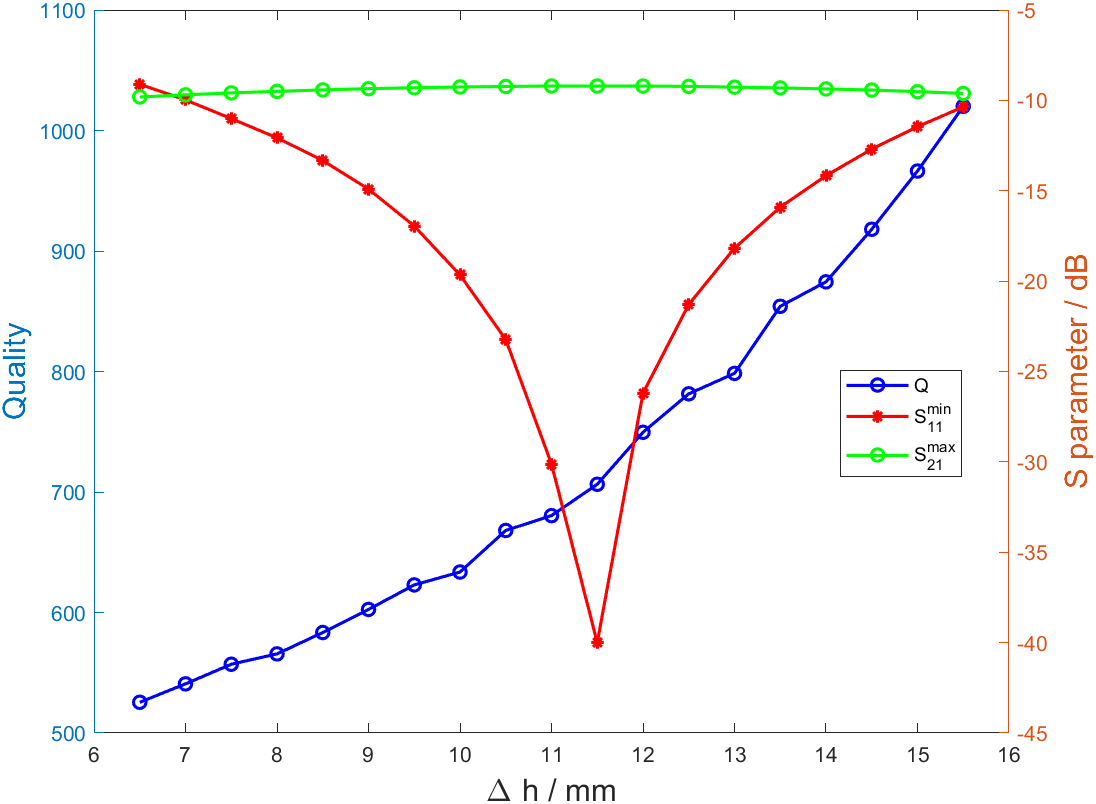
\includegraphics[width=0.8\linewidth]{helical/helical_coupling_delta}
    \caption[谐振腔耦合过程特性]{谐振腔耦合过程特性。横坐标为耦合线圈到主线圈的距离$\Delta h$,左侧和右侧的纵坐标分别是品质因子数值(单位1)和散射系数值(单位dB)。其中蓝色‘o’标线是谐振腔的品质因子Q,红色‘*’标线是相应的最佳耦合时的反射系数最小值$S_{11}^{min}$,绿色‘o’标线是相应的最佳耦合时的透射系数最大值$S_{21}^{max}$。\label{fig:helical_coupling_delta}}
\end{figure}

从上面的耦合过程结果来看,耦合线圈距离主线圈距离越远的情况下Q值越高。也就是说两者相互‘影响’越小的情况下Q值会越高。这个影响实际上就是等效的阻抗带来的耗散,为了验证这一点我们进行了另一组仅改变耦合线圈电阻值的实验,结果如图\ref{fig:helical_coupling_rin}所示。从图\ref{fig:helical_coupling_rin}中可以看出,随着耦合线圈电阻值的增加,Q值逐渐下降,同时也伴随着最佳耦合频率的偏移。不难发现,增加耦合线圈电阻值的过程这个结果跟图\ref{fig:helical_coupling_delta}中耦合线圈与主线圈距离的减小过程的结果是相互对应的。
\begin{figure}
    \centering
    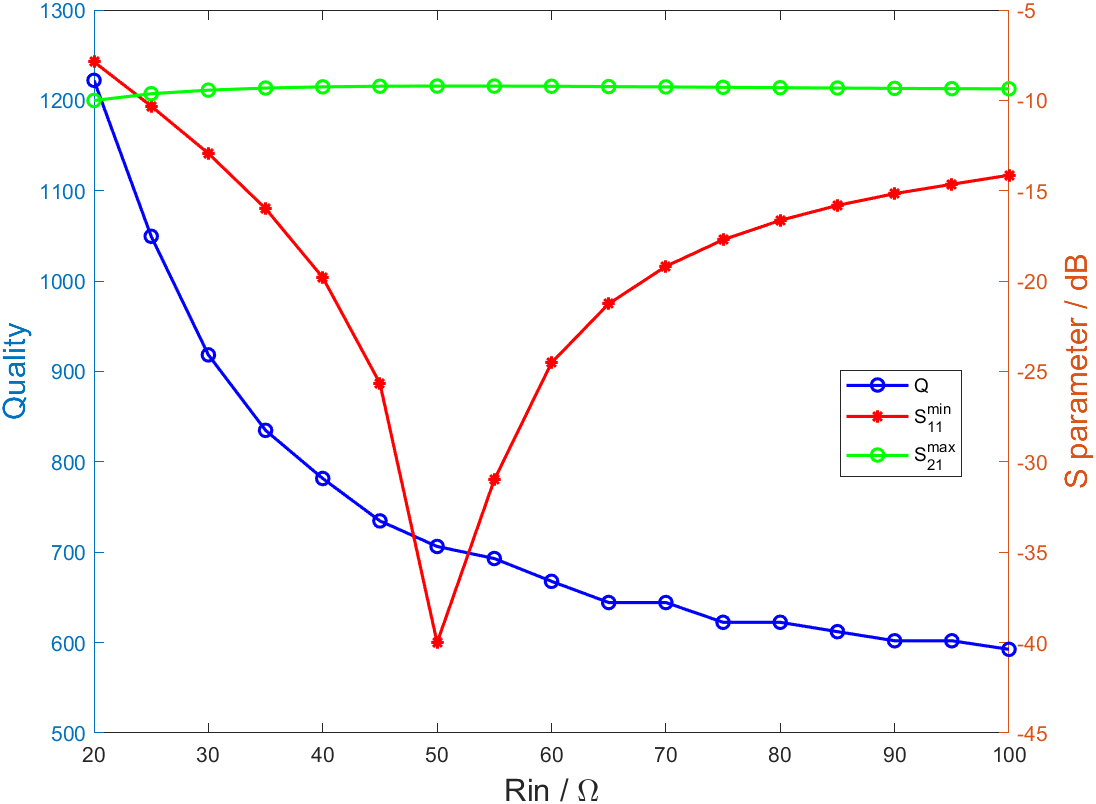
\includegraphics[width=0.8\linewidth]{helical/helical_coupling_rin}
    \caption[谐振腔耦合过程特性]{谐振腔耦合过程特性。横坐标为耦合线圈的阻值$R$,左侧和右侧的纵坐标分别是品质因子数值(单位1)和散射系数值(单位dB)。其中蓝色‘o’标线是谐振腔的品质因子Q,红色‘*’标线是相应的最佳耦合时的反射系数最小值$S_{11}^{min}$,绿色‘o’标线是相应的最佳耦合时的透射系数最大值$S_{21}^{max}$。\label{fig:helical_coupling_rin}}
\end{figure}


% \textcolor{red}{可以考虑将耦合过程会有不同的Q值的那个图也放上来说明一下\dots}

\newpage
\section[螺线管谐振腔的数学建模]{螺线管谐振腔的数学建模\label{section:helical_theory_model}}

螺线管谐振腔的集总电路模型可以解释和预测器件的行为。一个好的电路模型可以帮助研究人员轻松地设计具有特定属性的设备。在这里,对于螺线管谐振腔,谐振频率和较高的Q因子是最重要的两个指标。首先,对于谐振频率,我们假设额外的输出导线长度电容是频率误差发生的主要原因,如第\ref{section:helical_output_wire}节所述。

\begin{figure}
    \centering
    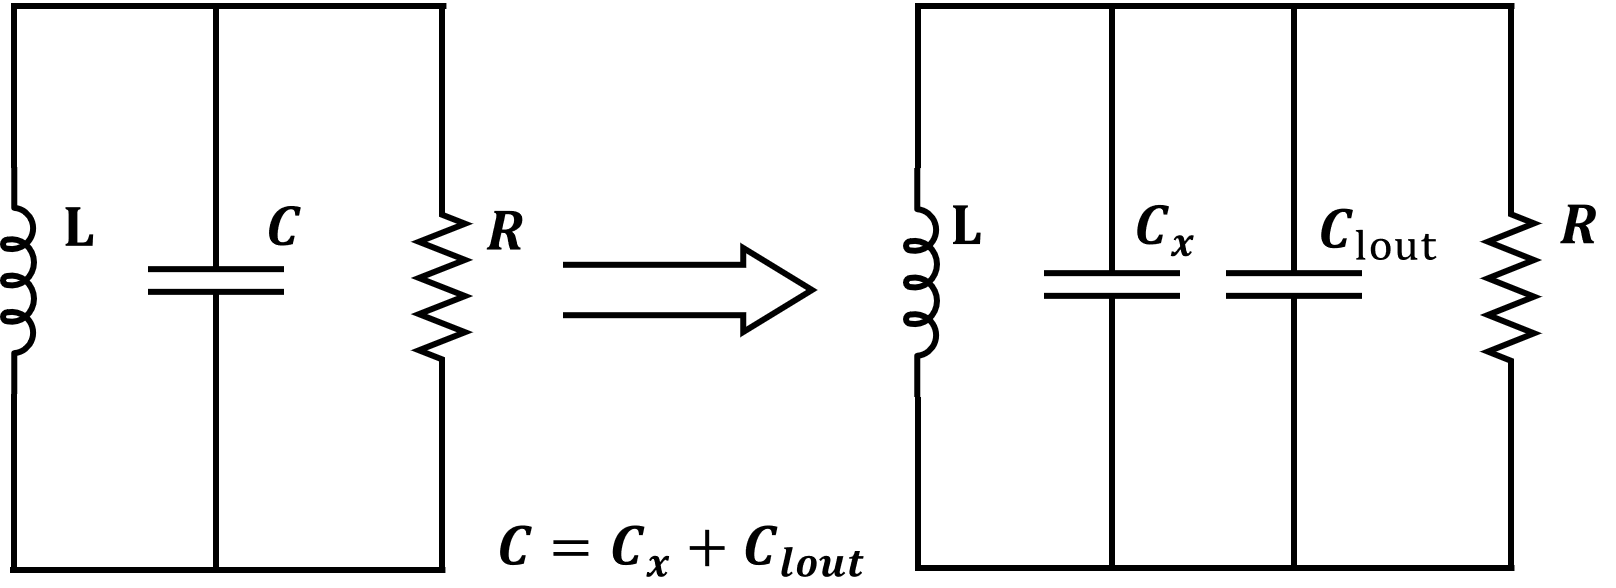
\includegraphics[width=0.8\linewidth]{helical/helical_RLC_circuit1}
    \caption[LCR电路模型]{LCR电路模型。$L$表示谐振腔的电感,主要包括耦合线圈和主线圈的电感;$R$表示整个谐振腔的电阻;$C$表示谐振腔的电容,$C_x$表示谐振腔内部结构的电容,$C_{lout}$表示谐振腔输出线引入的电容。\label{fig:helical_RLC_circuit1}}
\end{figure}

因此,输出线电容被添加到LCR电路模型中,如图\ref{fig:helical_RLC_circuit1}所示。总等效电容可视为传统电容CT和输出线总电容$C_{lout}$的总。传统的电容部分与以往的研究相同,而输出线和外部屏蔽将形成同轴电容:
\begin{align} 
	C_{lout}&=C_{lout1}+C_{lout2} \label{eq:helical_lout}\\ 
	C_{lout1}&=\frac{2\pi\epsilon_0 l_{out1}}{ln(D/d_0)} \label{eq:helical_lout1}\\ 
	C_{lout2}&=\frac{2\pi\epsilon_0 l_{out2}}{ln(D_1/d_0)} \label{eq:helical_lout2}
\end{align}

其中输出线电容$C_{lout1}$($C_{lout2}$)是长度为$l_{out1}$($l_{out2}$)的输出线与内径为$D$($D_1$)侧壁形成的电容。

然而,在补偿输出线长效应后,频率预测仍然低于数值模拟或实验结果。经过多次尝试,我们发现主要原因是对电容$C_c$和$C_s$的高估。最近的一项研究\cite[p52,f5.3]{article_2010}给出了一个螺线管电容$C_c$的新估计公式:
\begin{align}
    C_c=\frac{4\epsilon_0 b}{\pi}(1+k_c)/cos^2\psi 	\label{eq:helical_C_c_new}
\end{align}

其中$k_c=0.717439(d/b)+0.933048(d/b)^{3/2}+0.106(d/b)^2$,$d$是螺线管的直径,$b$是螺线管的长度,$\psi$是螺距角($\tan\psi=\tau/(\pi d)\approx 1$),$\epsilon_0$是真空介电常数。

另一方面,屏蔽壁电容$C_s$在主线圈和外部屏蔽壁之间形成,与电容$C_{lout}$相同,因此同轴电容公式可用于计算$C_s$。主线圈的等效同轴线长度为$Nd_0$,单匝等效长度为$d_0$,总主线圈有$N$匝,因此屏蔽电容计算为:
\begin{align}
    C_s=2\pi\epsilon_0 \frac{Nd_0}{ln(D/d')} \label{eq:helical_C_s_new}
\end{align}

其中$d'$是一个等效的线圈直径,$d'=d+\pi d_0/4$,其中$\pi d_0/4$是一个用于修正线圈边缘效应的因子。

此外,实际的主线圈螺旋长度有限,匝稀疏,因此需要更新或修改文献\cite[]{Siverns_Simkins_Weidt_Hensinger_2012}中的电感计算方法。短螺旋电感估计方法可计算为:
\begin{align}
    L=\frac{\mu_0 \pi (d/2)^2 }{\tau^2} (\sqrt{b^2+(d/2)^2}-d/2) \label{eq:helical_L_new}
\end{align}

\begin{figure}
    \centering
    \subcaptionbox[HUST模型结果]{HUST模型结果\label{fig:helical_freqmodelcompare_hust}}{
        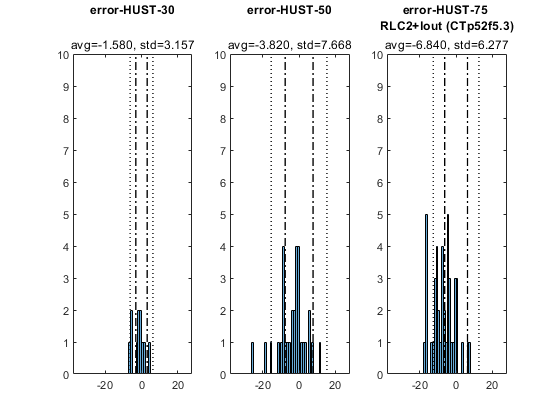
\includegraphics[width=0.55\linewidth]{helical/helical_freqmodelcompare_hust}
    }
    \subcaptionbox[Sussex模型结果]{Sussex模型结果\label{fig:helical_freqmodelcompare_sussex}}{
        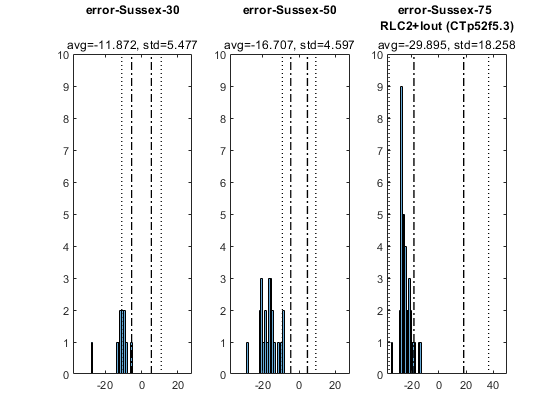
\includegraphics[width=0.55\linewidth]{helical/helical_freqmodelcompare_sussex}
    }
    \subcaptionbox[SUST模型结果]{SUST模型结果\label{fig:helical_freqmodelcompare_sust}}{
        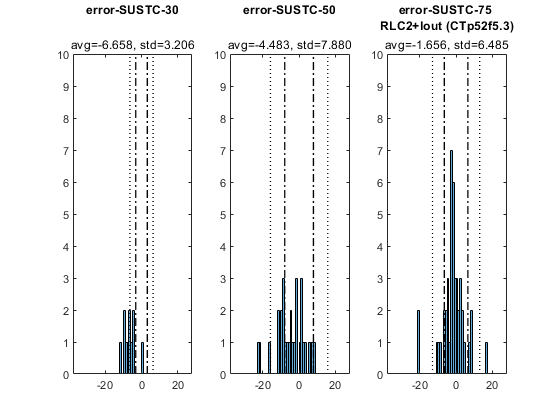
\includegraphics[width=0.55\linewidth]{helical/helical_freqmodelcompare_sust}
    }
    \caption[三种理论模型的预测效果比较]{三种理论模型的预测效果比较。左、中、右图分别是30 MHz、50 MHz、75 MHz附近频率设置的模型与参考表中偏差的结果的频数统计图。作为参考,每幅图上方给出了所有偏差的均值和其标准差。\label{fig:helical_freqmodelcompare}}

\end{figure}

最后,我们通过更新上述所有估计的方法,得到了一个新的频率预测模型。我们比较了频率预测模型、Sussex模型\cite[]{Siverns_Simkins_Weidt_Hensinger_2012}、SUST模型(本文)和 HUST模型\cite[]{Deng_Sun_Yuan_Xu_Zhang_Lu_Luo_2014}的准确性。
基于数值模拟结果,通过统计直方图对模型的有效性和准确性进行比较和评估,如图14(c)所示。频率误差的平均值和标准差越小,精度越好,误差离散越小。
所有的模型都与仿真的结果为标准做比较。
图\ref{fig:helical_freqmodelcompare}中的每一个数据结果都是一些列可行的$d,\tau$参数组合的模型预测和仿真结果的差值$\delta f=f_{model}-f_{HFSS}$,最终绘制出误差的统计分布。
针对不同的谐振频率组计算和模拟一系列离散的$d,\tau$参数(与表\ref{tb:helical_simulation_parameters}$30$ MHz、$50$ MHz、$75$ MHz)。$d$的样本在$20-80$ mm的范围内,步长为$10$ mm;$\tau$的样本在$4-18$ mm的范围内,步长为$2$ mm。
平均偏差和标准偏差都在每个图的顶部标记。平均值是一个有符号值,表示模型的整体频率预测效果。标准差表示频率误差的离散程度。


% \begin{figure}
%     \centering
%     \caption[HUST模型结果]{HUST模型结果\label{fig:helical_freqmodelcompare_hust}}
%     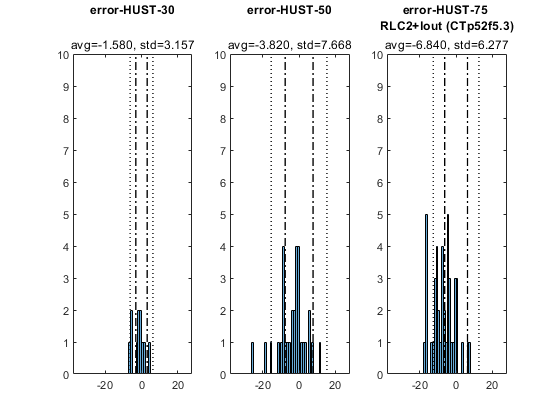
\includegraphics[width=0.33\linewidth]{helical/helical_freqmodelcompare_hust}
% \end{figure}

% \begin{figure}
%     \centering
%     \caption[Sussex模型结果]{Sussex模型结果\label{fig:helical_freqmodelcompare_sussex}}
%     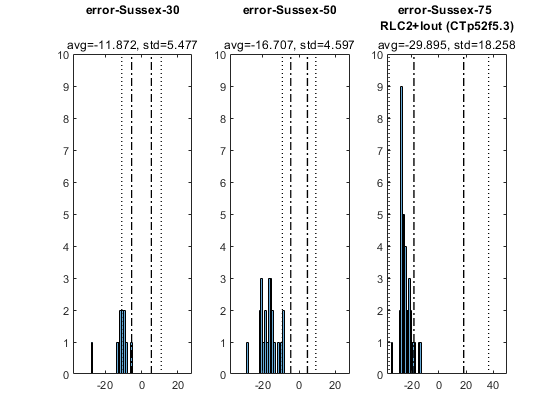
\includegraphics[width=0.33\linewidth]{helical/helical_freqmodelcompare_sussex}
% \end{figure}

% \begin{figure}
%     \centering
%     \caption[SUST模型结果]{SUST模型结果\label{fig:helical_freqmodelcompare_sust}}
%     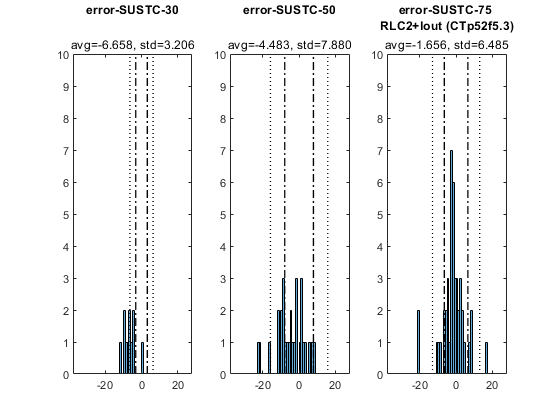
\includegraphics[width=0.33\linewidth]{helical/helical_freqmodelcompare_sust}
% \end{figure}

直方图结果表明:对于$75$ MHz组,本文中的模型的均值和标准差(SUST)在三个模型中都是最小的,预测的准确性是最好的。对于 $50$ MHz组,SUST和HUST模型之间的平均偏差值和标准偏差值基本相似。它们都预测了比Sussex模型更准确的谐振频率。对于$30$ MHz组,HUST频率预测的平均值最小,SUST模型准确率次之,但它们都优于Sussex模型。HUST和SUST模型的标准偏差相似,但它们都优于Sussex模型。需要注意的是,在$30$ MHz组中,由于主线圈线长度约束,所有$56$种可能组合中只有$11$个可行数据,参见式\eqref{eq:helical_fixed_constraints_1}和\eqref{eq:helical_fixed_constraints_2},因此结果可能会波动和偏差很大。

在上述结果中,对于$30-80$ MHz频率范围内的情况,本文提出的LCR模型提高了预测精度。输出线效应(参见第\ref{section:helical_output_wire}节)作为对分布式电容效应的替代解释,给出了更简单直观的物理解释。

\section[螺线管谐振腔的机械结构优化]{螺线管谐振腔的机械结构优化}

\subsection[惯用旧版谐振腔]{惯用旧版谐振腔}
惯用的旧版谐振腔设计如图\ref{fig:helical_old_design}所示。在该设计中,主线圈的接地/直流输入端口安装在谐振腔侧壁、即主屏蔽壳上。在采用以SMA为代表的射频连接头作为端口时,会产生额外的径向长度,导致配件之间的机械冲突,安装的时候主线圈很难直接放入外筒中。装配时一般需要先将输出头向内弯折,进入筒后再进行折回,将射频接头上紧固定;或者先将射频头固定在侧壁上,装入主线圈后再进行焊接。上述两种安装方式都缺乏便利性,比如弯折过程中射频连接头焊接会脱落、或壳内焊接的复杂度较高。更重要的是,安装时往往会破坏主线圈的结构,很难完全恢复到进筒前的结构参数。还有,该设计中对主线圈的支持较弱,主线圈易形变。这在装配时会导致难以将线圈按照目标设计参数准确地进行装配,增加调试成本。即使装配好了,在工作过程中也会对外界机械抖动等较为敏感、稳定性差。该设计的耦合方式也较为笨拙,在实际使用中需要花费大量时间来拆卸谐振腔、调整腔内小线圈的形状来实现最佳耦合。
除此之外,该设计的主线圈输出端口的便利性、稳定性以及屏蔽性能较差。为了减小金属电容板与线圈之间的等效电容影响,通孔直径较大,使得谐振腔的信号泄露增加、屏蔽效果减弱。而谐振腔在与后级设备进行连接时,通过中空螺柱进行压接连接,稳定性较差。
为此,我们设计了一款新的谐振腔来解决以上提到的一些问题。

\begin{figure}
    \centering
    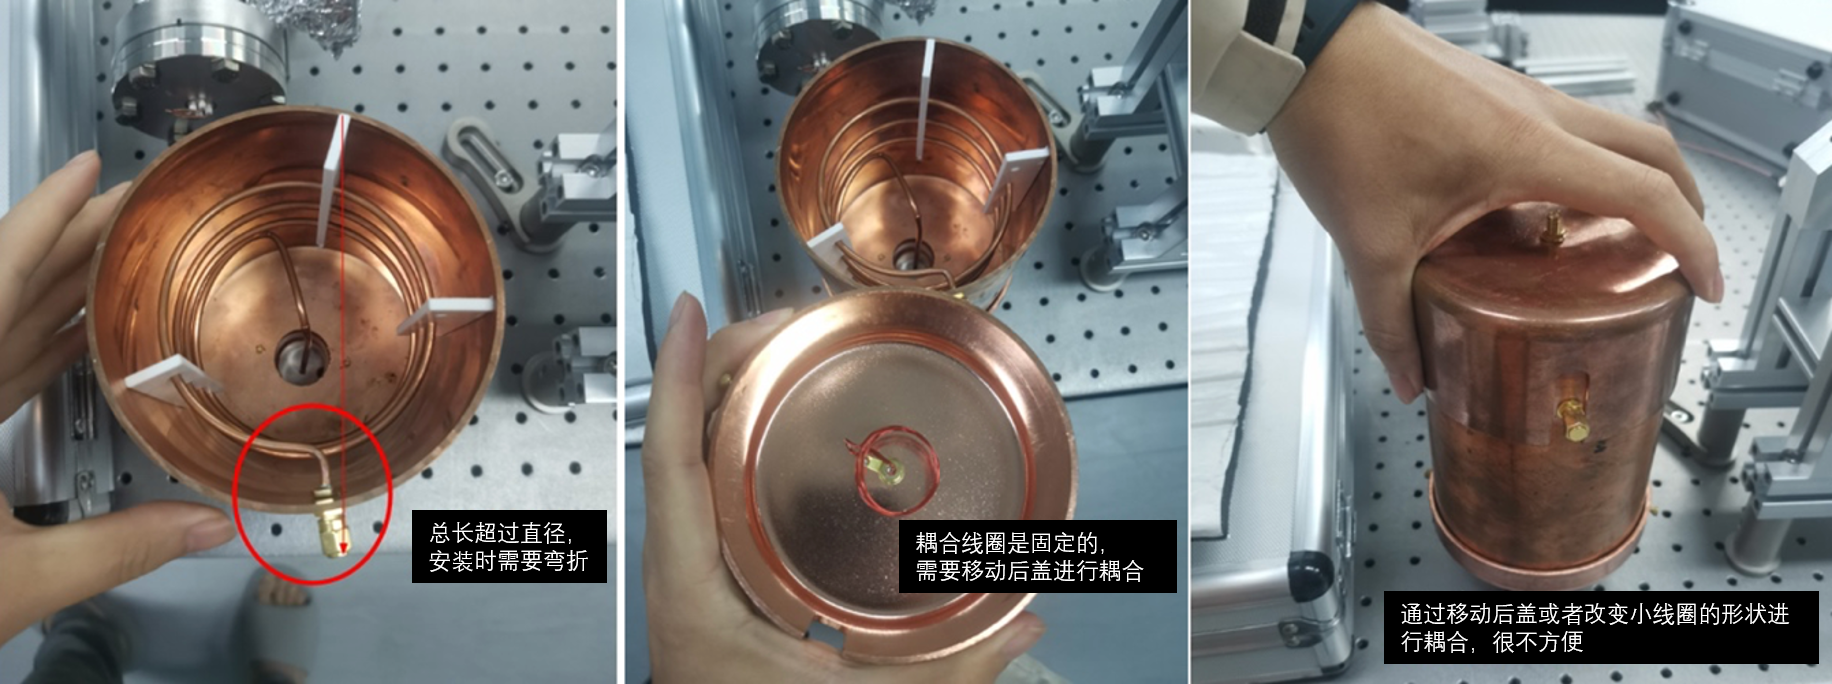
\includegraphics[width=1.0\linewidth]{helical/helical_old_design}
    \caption[旧版的谐振腔设计]{旧版的谐振腔设计,有机械冲突、耦合方式较差。\label{fig:helical_old_design}}
\end{figure}
\subsection[易装配易耦合的新版谐振腔]{易装配易耦合的新版谐振腔}
新的易装配易耦合的模块化谐振腔设计如图\ref{fig:helical_new_design}所示。它解决了现有技术对主线圈的安装较为不便、对主线圈固定的稳定性差、对次级线圈耦合部分缺乏灵活调节的问题。新的设计主要包括以下结构:
\begin{enumerate}
    \item 主腔体屏蔽与支撑部分,包括:主屏蔽壳、底部和顶部两个固定板(记为固定板一与固定板二)、四个固定柱、一个输出屏蔽壳;
    \item 线圈及其固定与调节结构,包括:一个或两个主线圈(以下图示说明均使用两个主线圈情况、但本结构同样适用于一个主线圈的情况)、一对主线圈固定支架、一个次级线圈、一个非旋转伸缩套筒、一个射频分压电路模块;
    \item 电学相关接口与紧固零件,包括:射频输入与输出接头、直流输入接头、射频分压输出接头、及若干固定螺丝。
\end{enumerate}

新设计的实物图如图\ref{fig:helical_new_design_real}所示,将主线圈的接地/直流输入端口转移至底部固定板一。安装时可以直接固定好底座,然后将主屏蔽壳套上,再盖上顶部的固定板,最后用四个固定柱将上下两个固定板连接起来即可。安装过程不存在装配上的机械冲突。
新设计采用一对主线圈固定支架对主线圈进行支撑与固定,通过固定支架上面的凹槽设计来约束线圈为目标参数(螺线的直径、螺距、长度)。这样在装配时易按照设计目标参数进行装配,在使用过程中也能够保持稳定。
新设计巧妙地采用了非旋转伸缩套筒来实现小线圈的平动耦合。非旋转伸缩套筒可实现高精度的平动,常用于光学系统中透镜的高精度调节。套筒中心可以用来固定射频接头,并与次级线圈连接,方便次级线圈的固定和外部信号输入。非旋转伸缩套筒的表面可以镀上氧化层,形成次级线圈部分与其它部分的绝缘,很好地隔离了两者,保证了次级线圈与主线圈仅通过自由空间进行耦合,接地部分不会相互干扰。
本设计通过主线圈末端焊接射频连接头、并固定至顶部固定板,来实现谐振腔的输出。该设计中,谐振腔主腔体几乎完全封闭,增加屏蔽效果,减少腔内信号泄露、以及腔外噪声的耦入。输出为标准射频接口,与后级设备连接的便利性更高,且稳定性也有了进一步的提升。

与现有技术相比,本设计设计更为合理,元件装配更加方便,谐振耦合更加精细快捷,谐振腔长时工作的稳定性更高。
\begin{figure}
    \centering
    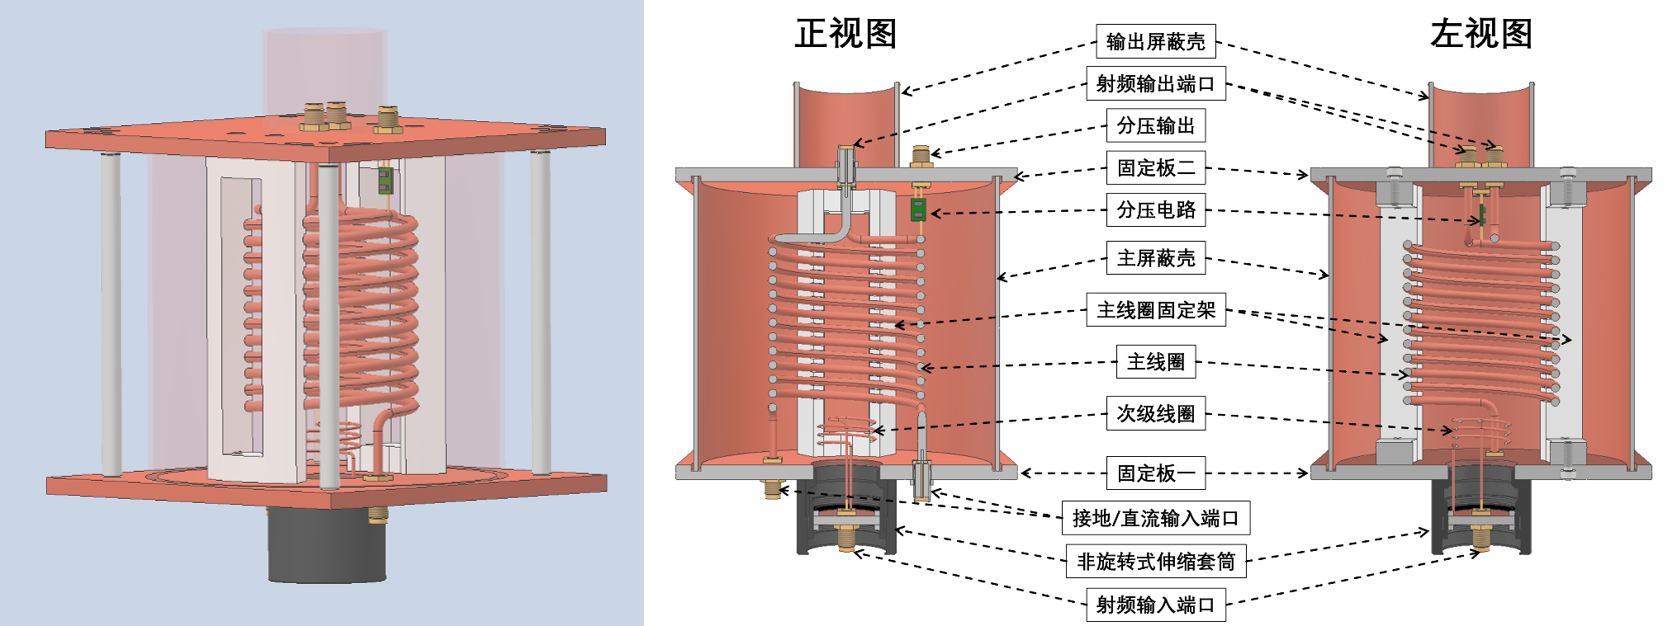
\includegraphics[width=1.0\linewidth]{helical/helical_new_design}
    \caption[易装配易耦合的谐振腔设计]{易装配易耦合的谐振腔设计\label{fig:helical_new_design}}
\end{figure}

\begin{figure}
    \centering
    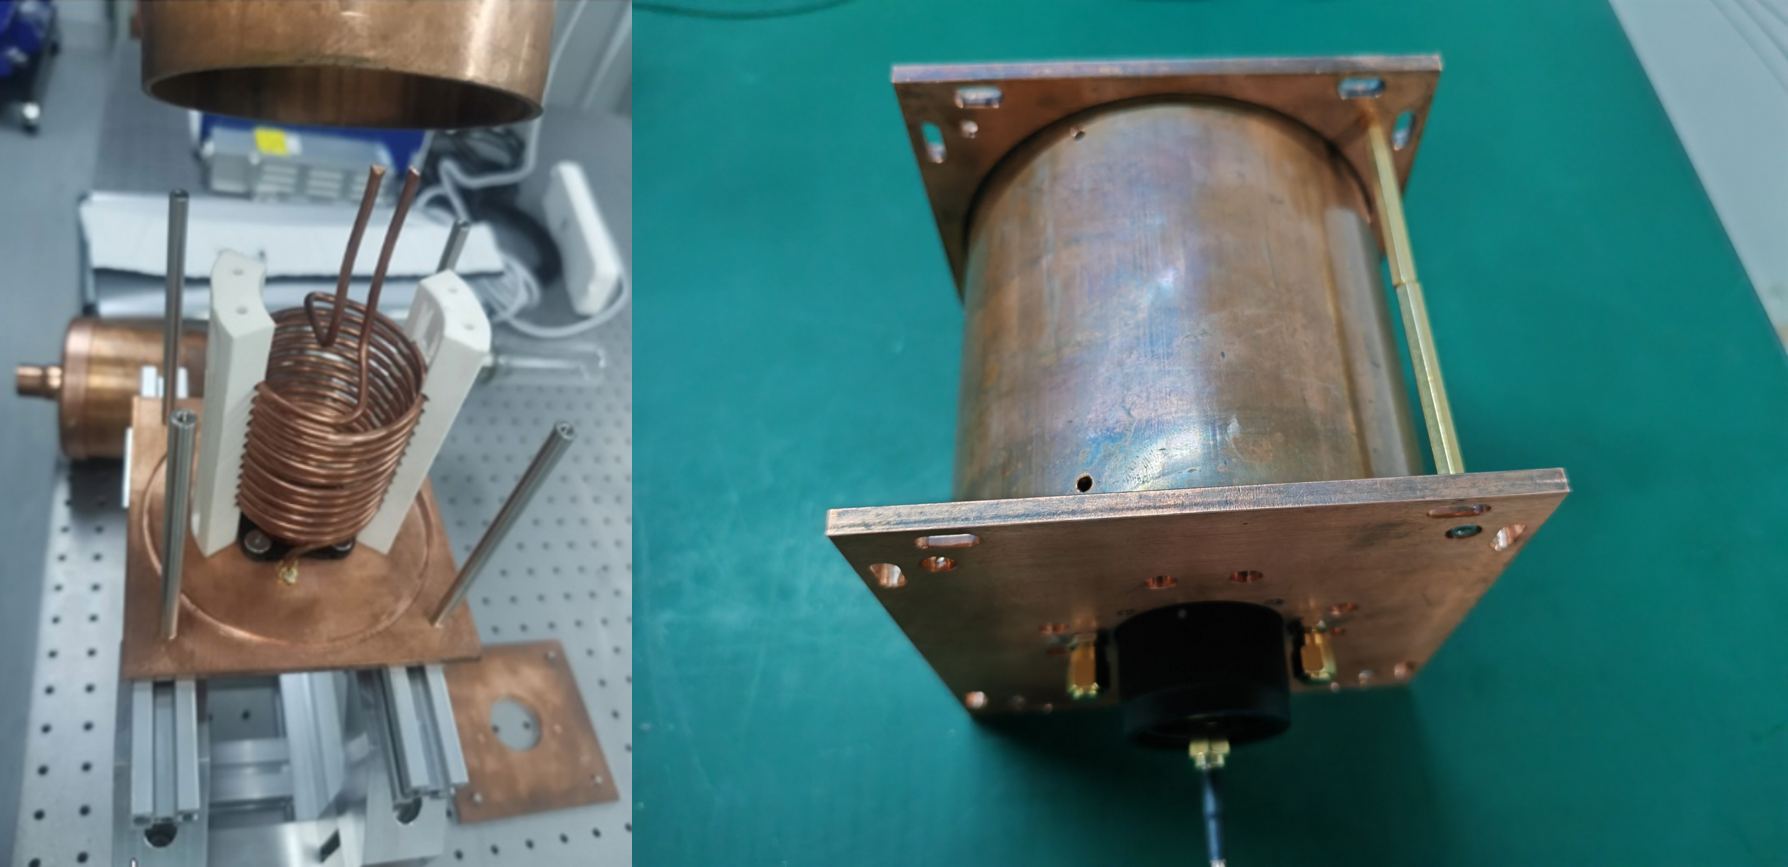
\includegraphics[width=1.0\linewidth]{helical/helical_new_design_real}
    \caption[易装配易耦合的谐振腔设计实物图]{易装配易耦合的谐振腔设计实物图\label{fig:helical_new_design_real}}
\end{figure}







\newpage
\section[章末小结]{章末小结}
螺线管谐振腔是离子阱系统中一种重要的射频器件,用于产生囚禁离子的射频信号。本章使用有限元(FE)仿真及实验相结合的方式研究了离子阱系统中的螺线管谐振腔的设计和加工问题。首先介绍了螺线管谐振腔在离子阱系统中的重要作用以及现有谐振腔设计的方式的问题和局限,接着使用商业有限元仿真软件HFSS建立了螺线管谐振腔的仿真模型,并且实际制作了若干组谐振腔进行了测试,通过将仿真结果与实验结果对比的方式验证了仿真模型的正确性和准确性。这一结果为谐振腔的进一步研究做好了准备,通过仿真预研的方式可以及大地方便对谐振腔各类物理参数变化的研究过程并且降低了研究成本。

Q值是谐振腔在离子阱量子计算系统中应用时关注的核心指标,更高的Q值能够带来更稳定的离子囚禁以及更高的离子比特保真度。本章接着针对适用于离子阱的特定频率范围的谐振腔Q值进行了优化研究,使用FE仿真的方式以紫铜材料为基础对谐振腔的各类几何结构参数变动对Q值和频率的影响进行了具体研究和分析。结果表明了主线圈的几何参数尤其是其直径、螺距和总线长是谐振腔性能最主要的影响因素。通过对谐振腔耦合过程特性的分析得出了用于耦合的小线圈几何参数对最佳耦合下的频率和Q值结果几乎没有影响,我们应将更多精力放在主线圈的设计和准确实现上。我们也从优化结果中找到了一组最优的几何参数进行了制作和测试并将其应用到了组内的离子阱实验系统中。

通过对螺线管谐振腔的仿真及实验数据结果的处理以及对谐振腔几何结构的分析,本章引入一种改进的LCR电路模型和新的电容评估公式给出了一个更加符合实际的谐振腔频率计算数学模型。相较于HUST和Sussex的数学模型结果,本章所给出的方法在多个频率段都有着更高的准确性。尽管通过数学模型计算得到的谐振腔频率与实际制作结果仍然存在差距,但是这种方式可以帮助研究者快速锁定大致几何参数范围,以更加高效快捷地使用仿真工具进行优化设计。
除此之外,对于实验系统中的谐振腔装配结构也进行了优化设计,给出了一种装配和耦合更方便且更加稳定的模块化谐振腔设计并制作和应用到了实验系统中,极大地促进了离子阱量子计算实验系统的稳定度和集成化。